\chapter{Design and construction of experimental apparatus}
\label{beamline}

\section{Introduction}
\label{intro_beamline}


\section{Beamline}
\label{sec:full_beamline}

\subsection{XUV Focusing}
\label{sec:XUV_focusing}

\begin{sidewaysfigure}
	\centering
	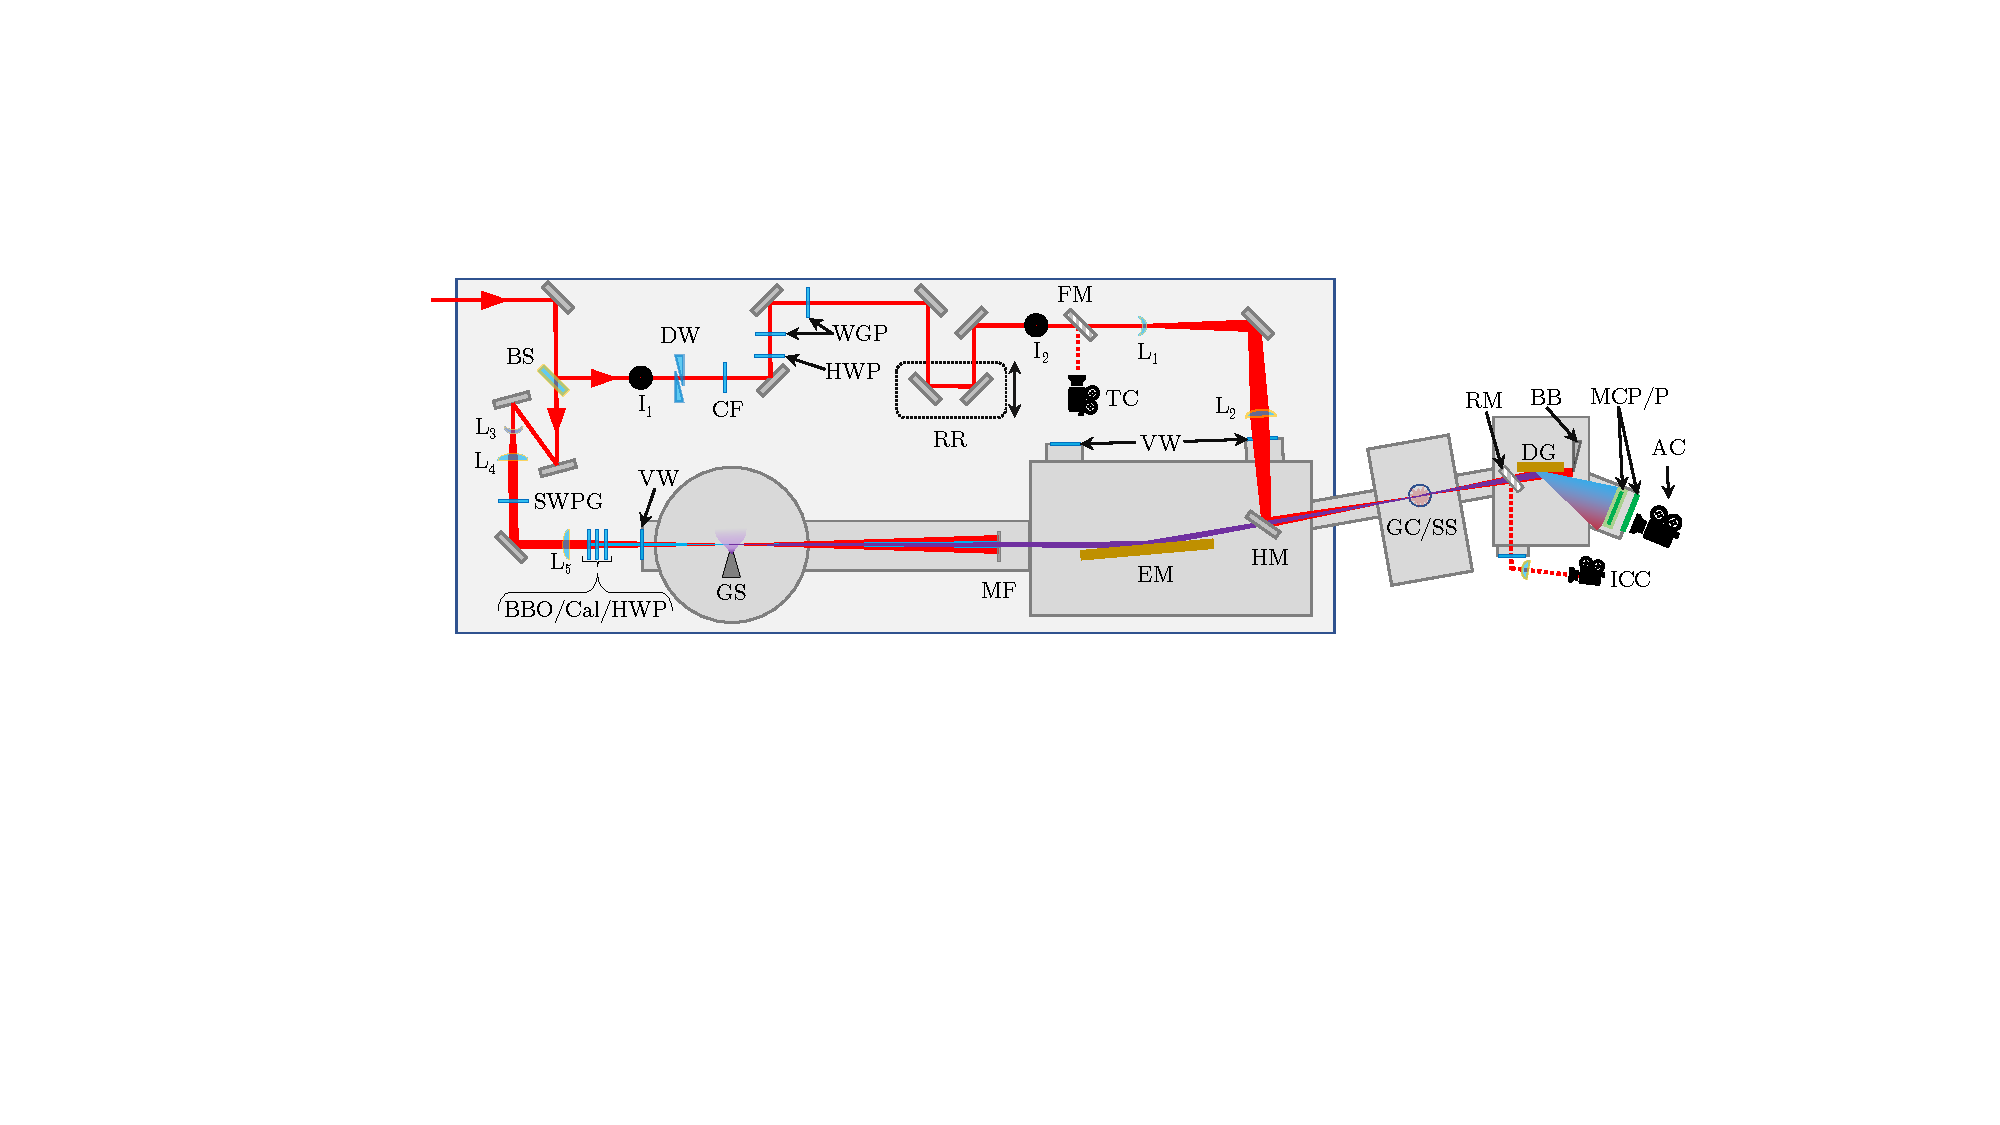
\includegraphics[width=1.0\textwidth]{figures/Beamline/beampath_sketch_3.pdf}
	\caption[Schematic of TABLe optical layout.]{Schematic of the beam path for the TABLe interferometer. The input laser is shown in red, its second harmonic in  blue, and the generated XUV in purple.  \textbf{BS}: Beamsplitter (Thorlabs BSF20-C), \textbf{I$_1$} and \textbf{I$_2$}: Irises used for alignment into interferometer. \textbf{DW}: Delay wedges for fine delay control, see section \ref{sec:delay_wedges}. \textbf{CF}: Color filter to remove parasitic colors from TOPAS (Thorlabs FELH1000). \textbf{HWP}: Half-wave plate. \textbf{WGP}: Wire grid polarizer. \textbf{RR}: Retro reflector for coarse delay adjustment.  \textbf{FM}: Flip mirror. \textbf{TC}: Thermal camera used for alignment.  \textbf{L$_1$}: $f=-300$ mm lens (Thorlabs LF1015-C). \textbf{L$_2$}: $f=500$ mm lens (Thorlabs LA1380-C). \textbf{VW}: Vacuum window, 3 mm CaF$_2$, \textbf{HM}: Hole mirror with 10 mm hole.  \textbf{L$_3$}: $f=-400$ mm lens.  \textbf{L$_4$}: $f=500$ mm lens. \textbf{SWPG}: Square-wave phase grating. \textbf{L$_5$}: $f=400$ mm lens.  \textbf{BBO}: Second-harmonic generation crystal.  \textbf{Ca}l: Calcite. \textbf{GS}: Gas source for HHG. \textbf{MF}: Metallic filter. \textbf{EM}: Ellipsoidal mirror. \textbf{GC/SS}: Gas cell or solid sample. \textbf{RM}: Removable mirror for \textit{in-situ} diagnotics.    \textbf{ICC}: camera for \textit{in-situ} diagnotics. \textbf{DG}: VLS diffraction grating. \textbf{BB}: Baffles to block zero order diffraction.  \textbf{MCP/P}: Microchannel plate and phosphor.  \textbf{AC}: Andor Neo 5.5 CMOS camera.}
	\label{fig:beampath_sketch}
\end{sidewaysfigure}


\subsection{Time Delay Control}
\label{sec:delay_wedges}

An important consideration in pump/probe experiments is how to control the delay between the pump and probe pulses.  To control this delay, there are typically two methods that can be employed optically.  The first to to use a retro-reflector that is mounted on a motorized stage \cite{jagerAttosecondTransientAbsorption2018, jagerAttosecondTransientAbsorption2017, bellTransientAbsorptionSpectroscopy2013, jiangChargeCarrierDynamics2015, borjaElectronDynamicsSolids2016, chengAttoseondTransientAbsorption2015}.  With this method, the delay is simply related to the displacement of the motorized stage by the relationship $\Delta\tau = 2\Delta x/c$.  This means that a displacement of 10 nm by the motorized stage would lead to a delay of 67 as, whereas a displacement of 2 in. would lead to a delay of 339 ps. This setup is advantageous if large delays are required (10s of ps to a few ns), however for the short time steps that are required for an attosecond measurement (typically on the order of 100 as) the requirements on the motor being used to move the retro are very high.  Since a 100 as step would equate to a translation of 15nm, this would require the use of a piezoelectric motor.  Piezo motors and their associated electronics tend to be expensive, and they have inherent problems because they exhibit nonlinear movement due to hysteresis and they tend to drift and creep after actuation.  This can be abated through a feedback sensor and operating it in a closed-loop mode, however the quality of the sensor and electronics determines how effectively these problems are minimized.

\begin{figure}
	\centering
	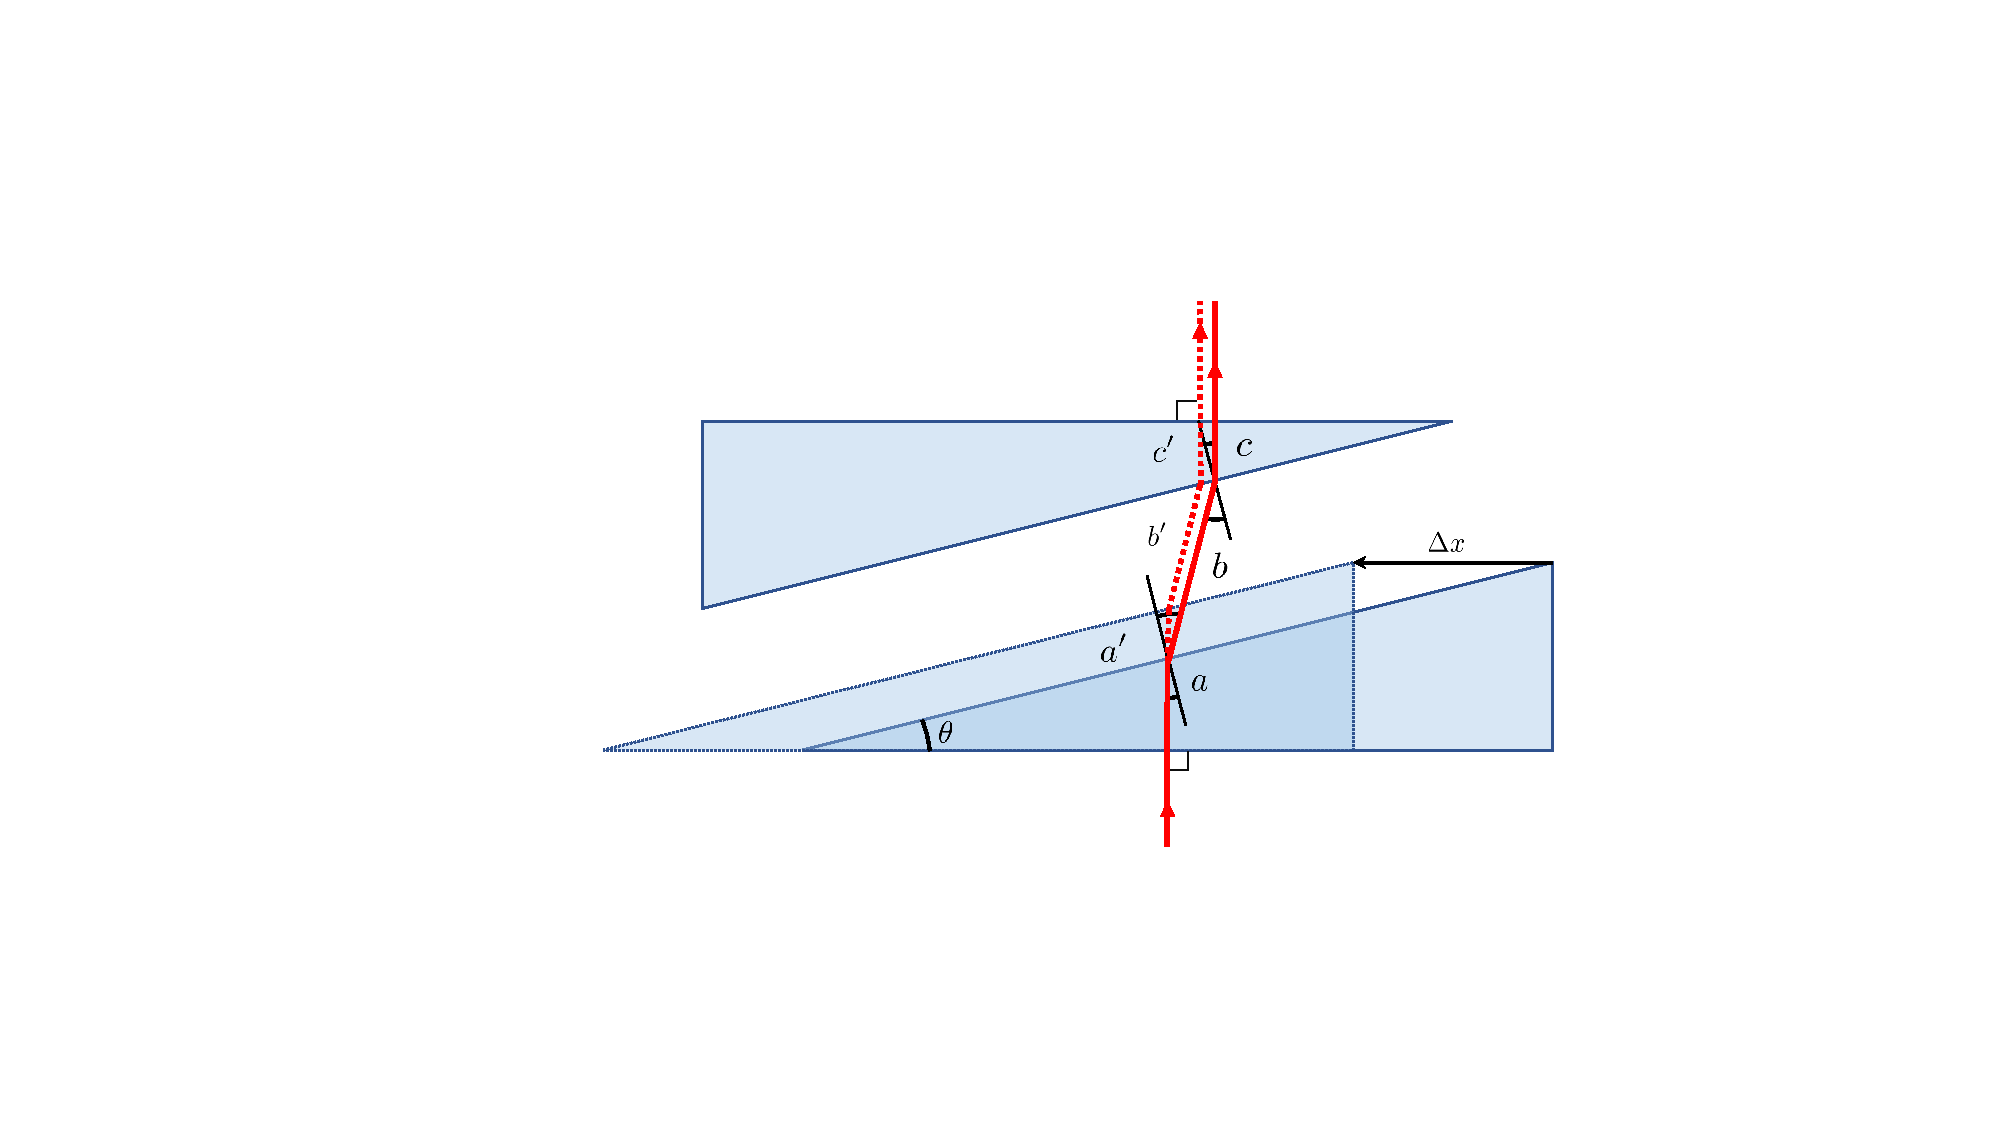
\includegraphics[width=0.8\textwidth]{figures/Beamline/wedge_delay_calibration.pdf}
	\caption[Schematic of FS wedges used for delay control]{Schematic of the FS wedges used to control the time delay between the IR and XUV pulses in the dressing and generation arms interferometer, respectively. The wedges are aligned such that the input beam is normal to the first wedge face, and the beam exits the wedges normal to the last face of the second wedge.  Only one of the wedges is motorized and is shown before and after a displacement by an amount $\Delta x$.}
	\label{fig:wedges}
\end{figure}

The second common method to control the delay between the pump and probe pulse is to use a pair of glass wedges \cite{chirlaAttosecondPulseGeneration2011, gormanAttosecondProbingElectron2018, kiesewetterDynamicsNearThresholdAttosecond2019}. A schematic of how this is achieved is shown in figure \ref{fig:wedges}.  In this scheme, only one of the glass wedges is motorized, and the direction of translation is perpendicular to the input beam and parallel to the first glass face.  The path that a ray would take through the wedge pair is shown before ($a\rightarrow b\rightarrow c$) and after ($a' \rightarrow b'\rightarrow c'$) translation by an amount $\Delta x$.  Assuming that the wedge angle is $\theta$, the path after translation by $\Delta x$ can be written as
\begin{align}
\label{eqn:path_lengths}
	a'&=a+\Delta x \tan\theta\\
	b'&=b-\Delta x \bigg(\frac{\sin\theta}{\cos\psi}\bigg)\\
	c'&=c+\Delta x \tan\theta\bigg(\frac{\sin(\psi-\theta)}{\cos\theta}\bigg)
\end{align}
where
\begin{equation}
	\psi = \arcsin(n\sin\theta)
\end{equation}
is given by Snell's Law \cite{pedrottiIntroductionOptics2007}. From the difference in optical path length between these two paths, one can calculate the time delay $\Delta\tau$ introduced by a translation of $\Delta x$, and this relationship is given by
\begin{equation}
\label{eqn:time_delay}
	\Delta\tau = \frac{\Delta x}{c}\Bigg[n\tan\theta - \frac{\sin\theta}{\cos\psi}-n\tan\theta\bigg(\frac{\sin(\psi-\theta)}{\cos\theta}\bigg)\Bigg].
\end{equation}
For a pair wedges made out of fused silica (Infrasil) with a wedge angle of $\theta=4^\circ$ and a beam of wavelength 1430 nm (n=1.4454), equation \ref{eqn:time_delay} becomes
\begin{equation}
\label{eqn:numerical_relationship_wedges}
	\Delta\tau = \Bigg(114 \bigg[\frac{\mathrm{as}}{\mathrm{\mu m}}\bigg]\Bigg)\Delta x.
\end{equation}
This entails that a translation of 1 $\mu$m would lead to a delay of only 100 as.  This reduction in motor step to delay step ratio compared to the retroreflector case means that the requirements on the motorized stage are greatly reduced.  Additionally, since the glass wedges are a transmissive optic, they are inherently less sensitive to vibrations when compared to a retroreflector.

In the TABLe apparatus, both types of delay control have been implemented, as shown in figure \ref{fig:beampath_sketch}.  The retroreflector is mounted on a translation stage with 2 inches of travel that is controlled manually with a micrometer.  The primary use for the retroreflector is to make coarse adjustments to the dressing arm to account for changes in temporal overlap between the two arms of the interferometer.  Typically, this is due to adjustments made to the interferometer itself (such as introducing new optics) or due to changes in the input laser, usually either pointing or wavelength.  

To finely control the delay, a pair of glass wedges is used.  These wedges are made out of fused silica, and have a wedge angle of $\theta=5^\circ$.  The first of the two wedges are motorized in manner similar to that shown in figure \ref{fig:wedges}.  The stage that the first wedge is mounted to has a total travel of 1 inch, and it is controlled by a Thorlabs Z825B DC servo motor.  This "pencil" motor, as it is known in the lab, has a minimum repeatable incremental motion of 0.2 $\mu$m and is encoded, so it's absolute position is known to within the homing accuracy of $\pm1$ $\mu$m.  From equation \ref{eqn:numerical_relationship_wedges}, using these wedges at 1430 nm with a step size of 1 $\mu$m will give a delay of 101 as.


\subsection{IR Dressing Intensity}
\label{sec:dressing_intensity}

An important consideration in any ATS experiment is the intensity of the IR field that is used as a probe/dressing field. Ideally, one would like to be able to control the intensity such that both perturbative and strong-field regimes can be accessed with the same optical setup.  This can be achieved by selecting an optical setup that has a high peak intensity and then attenuate the beam 
to achieve a lower intensity.  Attenuation can be achieved through the use of neutral density (ND) filters, however they can lead to several complications.  Since the ND filter would be placed in only one arm of the interferometer to control only the dressing intensity, any variation in thickness between different ND filters would lead to a change in temporal overlap.  Additionally, any change in positioning when switching ND filters will lead to a slight change in spatial overlap. In light of this, the method to attenuate the beam that was implemented in the TABLe interferometer is a half-wave plate (HWP) and a wire grid polarizer (WGP).  By rotating the polarization using the HWP, we can finely control the intensity  of the dressing field by using the WGP to transmit only one component of the rotated polarization.  The WGP is set such that the initial polarization is maintained, and this insures that the polarization of the IR and XUV are parallel in the interaction region.  A second WGP is used to increase the effective extinction ratio to ensure that the field is linearly polarized even when it is being strongly attenuated.  The extinction ratio of one of the WGP (Thorlabs WP25M-UB) is approximately 12500:1 at 1430 nm.  Using this setup in conjunction with a beam splitter that reflects 8\% of the input energy to the dressing arm, the pulse energy can be tuned between 1 $\mu$J and 125 $\mu$J.

\begin{figure}
	\centering
	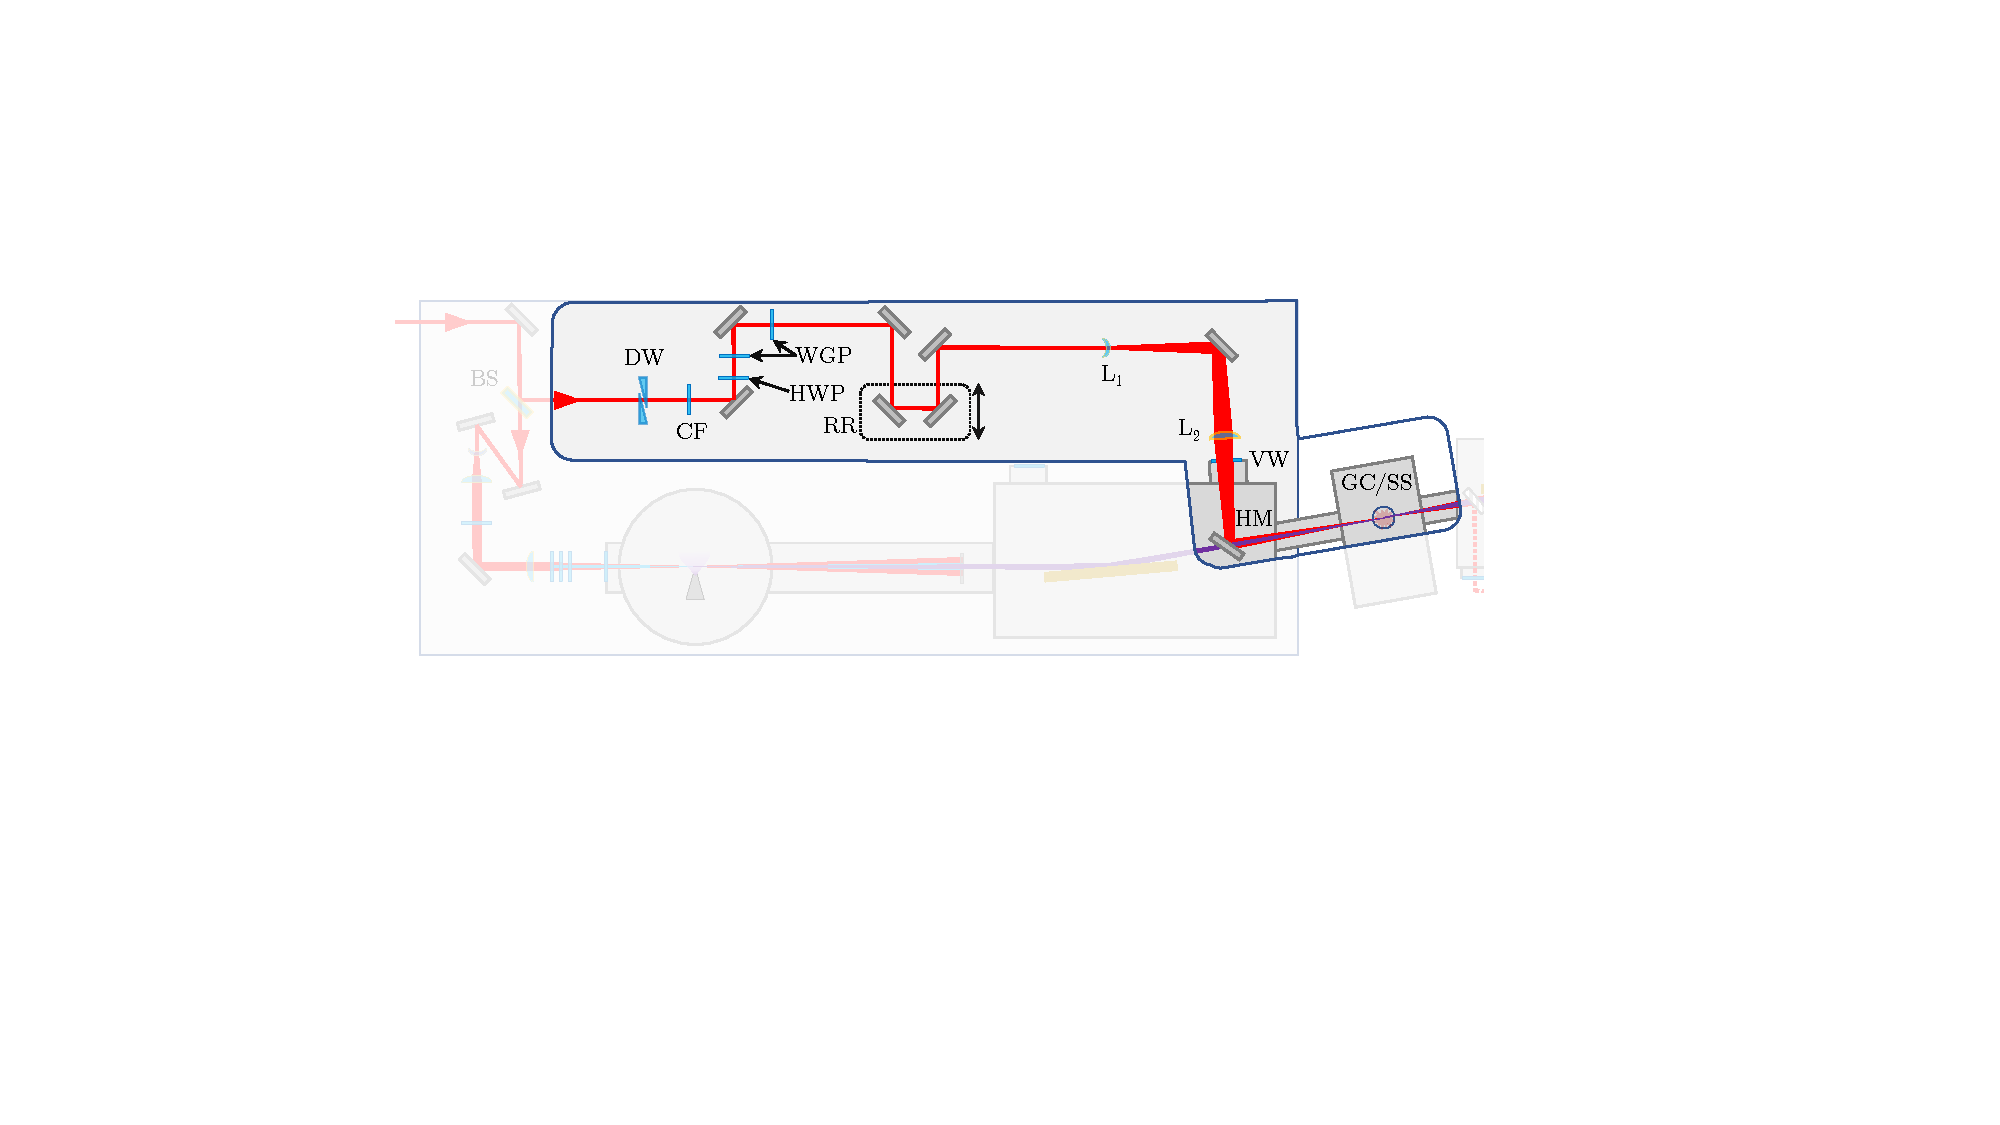
\includegraphics[width=0.9\textwidth]{figures/Beamline/dressing_arm.pdf}
	\caption[Optical layout of dressing arm]{Optical layout of the dressing arm of the TABLe interferometer. HWP and WGP are used to finely control the power in the dressing arm.  The lenses L$_1$ and L$_2$ were chosen to achieve a high intensity at the focal plane in the target chamber.  This was done to have the capability to drive stong-field processes in a gas medium \cite{kiesewetterDynamicsNearThresholdAttosecond2019}.  See figure \ref{fig:beampath_sketch} for full details of the interferometer.}
	\label{fig:dressing_arm}
\end{figure}

The next design consideration for the dressing arm of the interferometer is choosing focusing optics to set the peak intensity that is achievable at the interaction region.  The two main options in this regard are either focusing mirrors or lenses.  Focusing mirrors have a significant advantage in the fact that they are achromatic, however their use leads to an optical system that is generally larger in optical path length and is difficult to switch between focal geometries. Lenses in that regard are well suited to adjusting between different experimental requirements without changing the overall footprint of the interferometer.  The dressing lenses that are used in all of the experiments in this dissertation are shown in \ref{fig:dressing_arm}, and they were originally selected to achieve the highest possible intensity at the focal plane given the geometrical constraints of the TABLe \cite{kiesewetterDynamicsNearThresholdAttosecond2019}. This choice of lenses was made to drive strong-field processes in rare gas atoms in the interaction region, and they were selected based upon calculations done by D. Kiesewetter using a hole mirrors as both beam splitters in the interferometer. His calculations estimated that the peak intensity at 1300 nm was 0.59 TW/cm$^2$ for a pulse energy of 1 $\mu$J just before L$_1$ in figure \ref{fig:dressing_arm}.

\begin{sidewaysfigure}%[ht]
	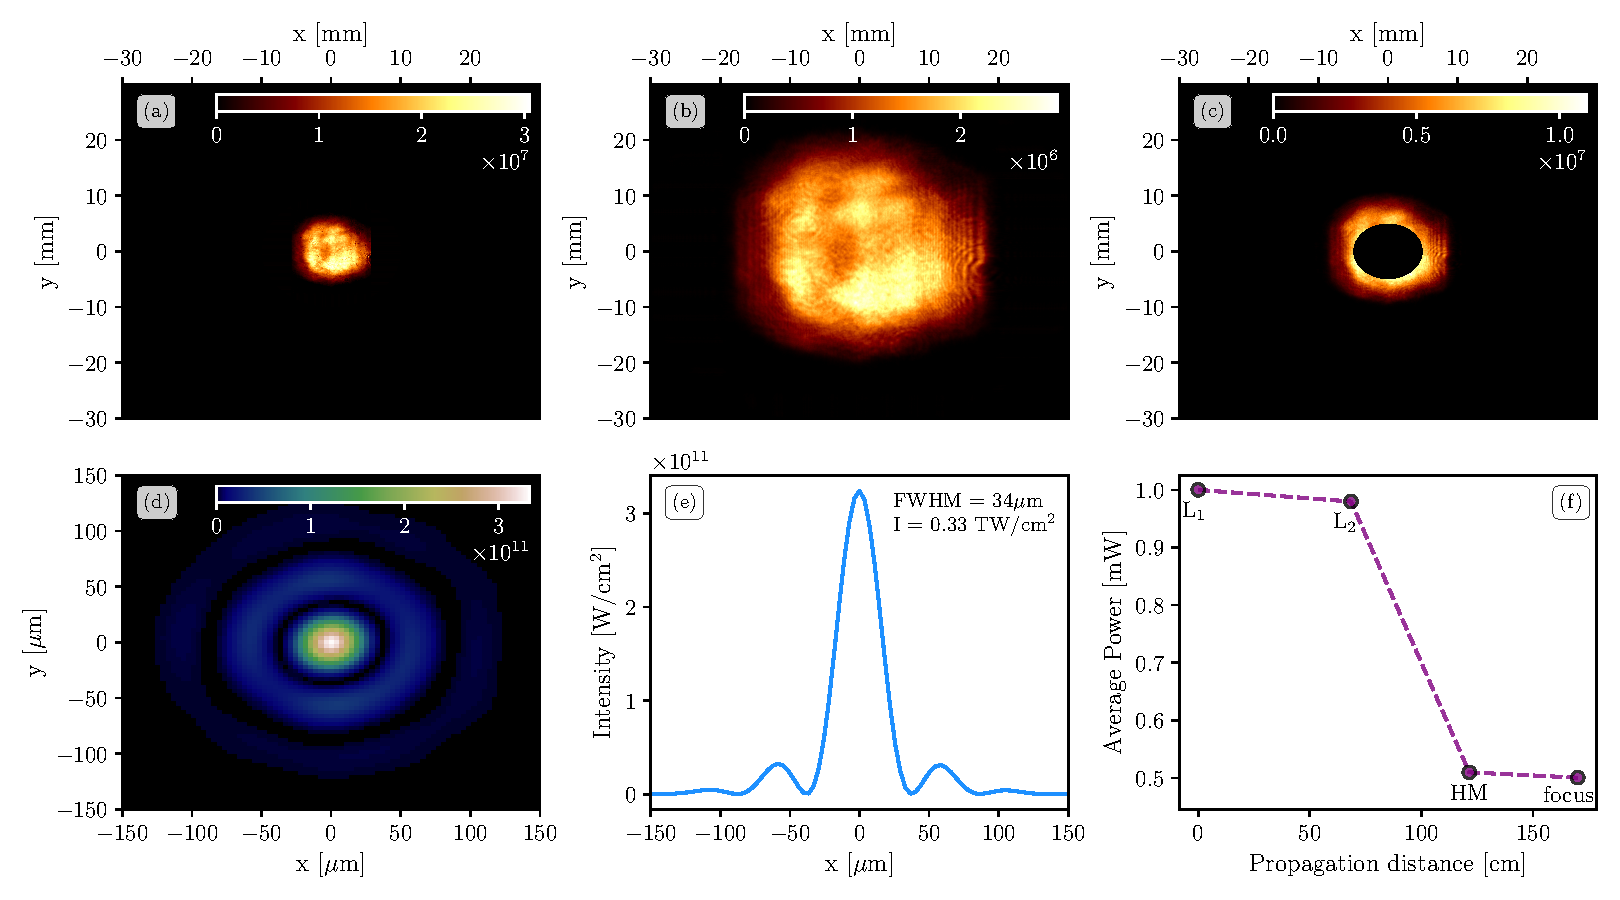
\includegraphics[width=\textwidth]{figures/Beamline/pump_intensity_profiles_1430nm_1uj.pdf}
	\caption[Calculation of dressing intensity]{(a) Beam profile of the signal from the TOPAS pumped by the Spitfire laser system.  Wavelength is 1430 nm and the pulse is normalized to 1 $\mu$J of pulse energy.  Beam profile was measured using a thermal camera, and is used as the input to the beam propagation simulation that is initiated just before L$_1$ in figure \ref{fig:dressing_arm}. (b) Numerically propagated beam profile just after L$_2$ in figure \ref{fig:dressing_arm}. (c) Beam profile just after reflecting off the hole mirror.  (d) Calculated intensity profile at the focal plane in the interaction region. (d) Lineout of the calculated intensity profile.  For an input pulse energy of 1 $\mu$J, a peak intensity of 0.33 TW/cm$^2$ can be achieved.  (f) Integrated average power at different point in the calculation.  The main source of energy loss is due to the hole mirror, which only reflects 52\% of the incident light.  The hole mirror has an inner radius of 5 mm in this case.}
	\label{fig:dressing_intensity}
\end{sidewaysfigure}


For the experiments described herein, the initial beam splitter was changed to a beam sampler and the recombining hole mirror was changed to a hole diameter of 10 mm from 6 mm.  This was done to maximize the XUV flux by sending as much energy to generation as possible while minimizing clipping of the XUV with the hole mirror.  In light of these changes, it is important to determine what the new peak intensity is at the focus.  To accurately determine the intensity, a beam propagation simulation is performed using the measured beam profile.  It is important to use the measured beam profile because the spatial mode out of the TOPAS is decidedly non-Gaussian, and this can be seen in \ref{fig:dressing_intensity} (a) which shows the beam profile at 1430 nm measured on a thermal camera.  Beam propagation is implemented using an open-source Python package developed by Flexible Optical B.V. (OKO Tech) called LightPipes.  The package consists of numerical methods to calculate the Fresnel integral
\begin{equation}
\label{fresnel_integral_0}
u(x,y,z)=\frac{i k}{2\pi z}e^{i k z}e^{i k (x^2+y^2)/2z}\int_{-\infty}^{\infty}\int_{-\infty}^{\infty}u(\xi,\eta,0) e^{ik(\xi^{2}+\eta^{2})/2z} e^{-ik(x\xi + y\eta)/z} \diff\xi\diff\eta
\end{equation}
which gives the field $u(x,y,z)$ after propagation of a distance $z$, given an initial field profile of $u(x,y,0)$.  Using this formalism, a thin lens of focal length can be treated as adding a quadratic phase $\phi=-\pi(x^2+y^2)/\lambda f$ to the field, and the effect of apertures can also be included to account for the effect of diffraction on the beam profile and intensity \cite{goodmanIntroductionFourierOptics2005}.

The results of the simulation are shown in figure \ref{fig:dressing_intensity}.  This simulation was performed for an input pulse energy of 1 $\mu$J at a wavelength of 1430 nm. The simulation begins just before L$_1$ in \ref{fig:dressing_arm} and the beam is propagated through to the interaction region GC/SS.  The beam profile at L$_2$ and immediately after the hole mirror is shown in figure \ref{fig:dressing_intensity} (b) and (c), and the intensity profile at the focus is shown in figure \ref{fig:dressing_intensity} (d).  From these simulations, the peak intensity for a pulse energy of 1 $\mu$J is 0.33 TW/cm$^2$. For the range of pulse energies available in the dressing arm, this corresponds to an intensity range of 0.33 - 413 TW/cm$^2$ that is achievable.

\subsection{XUV Beam Size}
\label{sec:xuv_beam_size_knife_edge}

An important consideration in any pump/probe experiment is the beam size of the probe relative to the pump in the interaction region.  The reason for this is because the probe beam inherently samples the excited state of the system induced by the pump at intensities within the intersection of the pump and probe focal volumes contained within the system being studied.  Thus, a smaller probe waist relative to the pump waist means that a narrower distribution of pump intensities will be sampled by the probe.  The width of this distribution limits the ability to study intensity dependent effects, and it is a critical parameter to control. As stated in section \ref{sec:XUV_focusing}, the demagnification of the XUV spot size provided by the ellipsoidal mirror helps tremendously to achieve as small ratio of probe to pump beam sizes even at small pump beam sizes that are used.

Additionally, it is also of great importance to place the sample at the focus of both the XUV and the IR beams in the target chamber.  This can be done easily with the IR either through direct imaging of the beam or by using an intensity dependent effect (such as second harmonic generation from a BBO) to find the peak intensity along the k-direction of the IR beam.  The focus of the XUV is more difficult to find because it must be found in vacuum.  One method to find the focus is to measure the beam diameter at various points along the k-direction of the XUV to find the minimum beam diameter.  A method to do this is to employ a knife-edge measurement \cite{arnaudTechniqueFastMeasurement1971, skinnerMeasurementRadiusHighpower1972,marshallTwoMethodsMeasuring2010,almeidaHarmonicsBeamsCharacterization2016}.

\begin{figure}
	\centering
	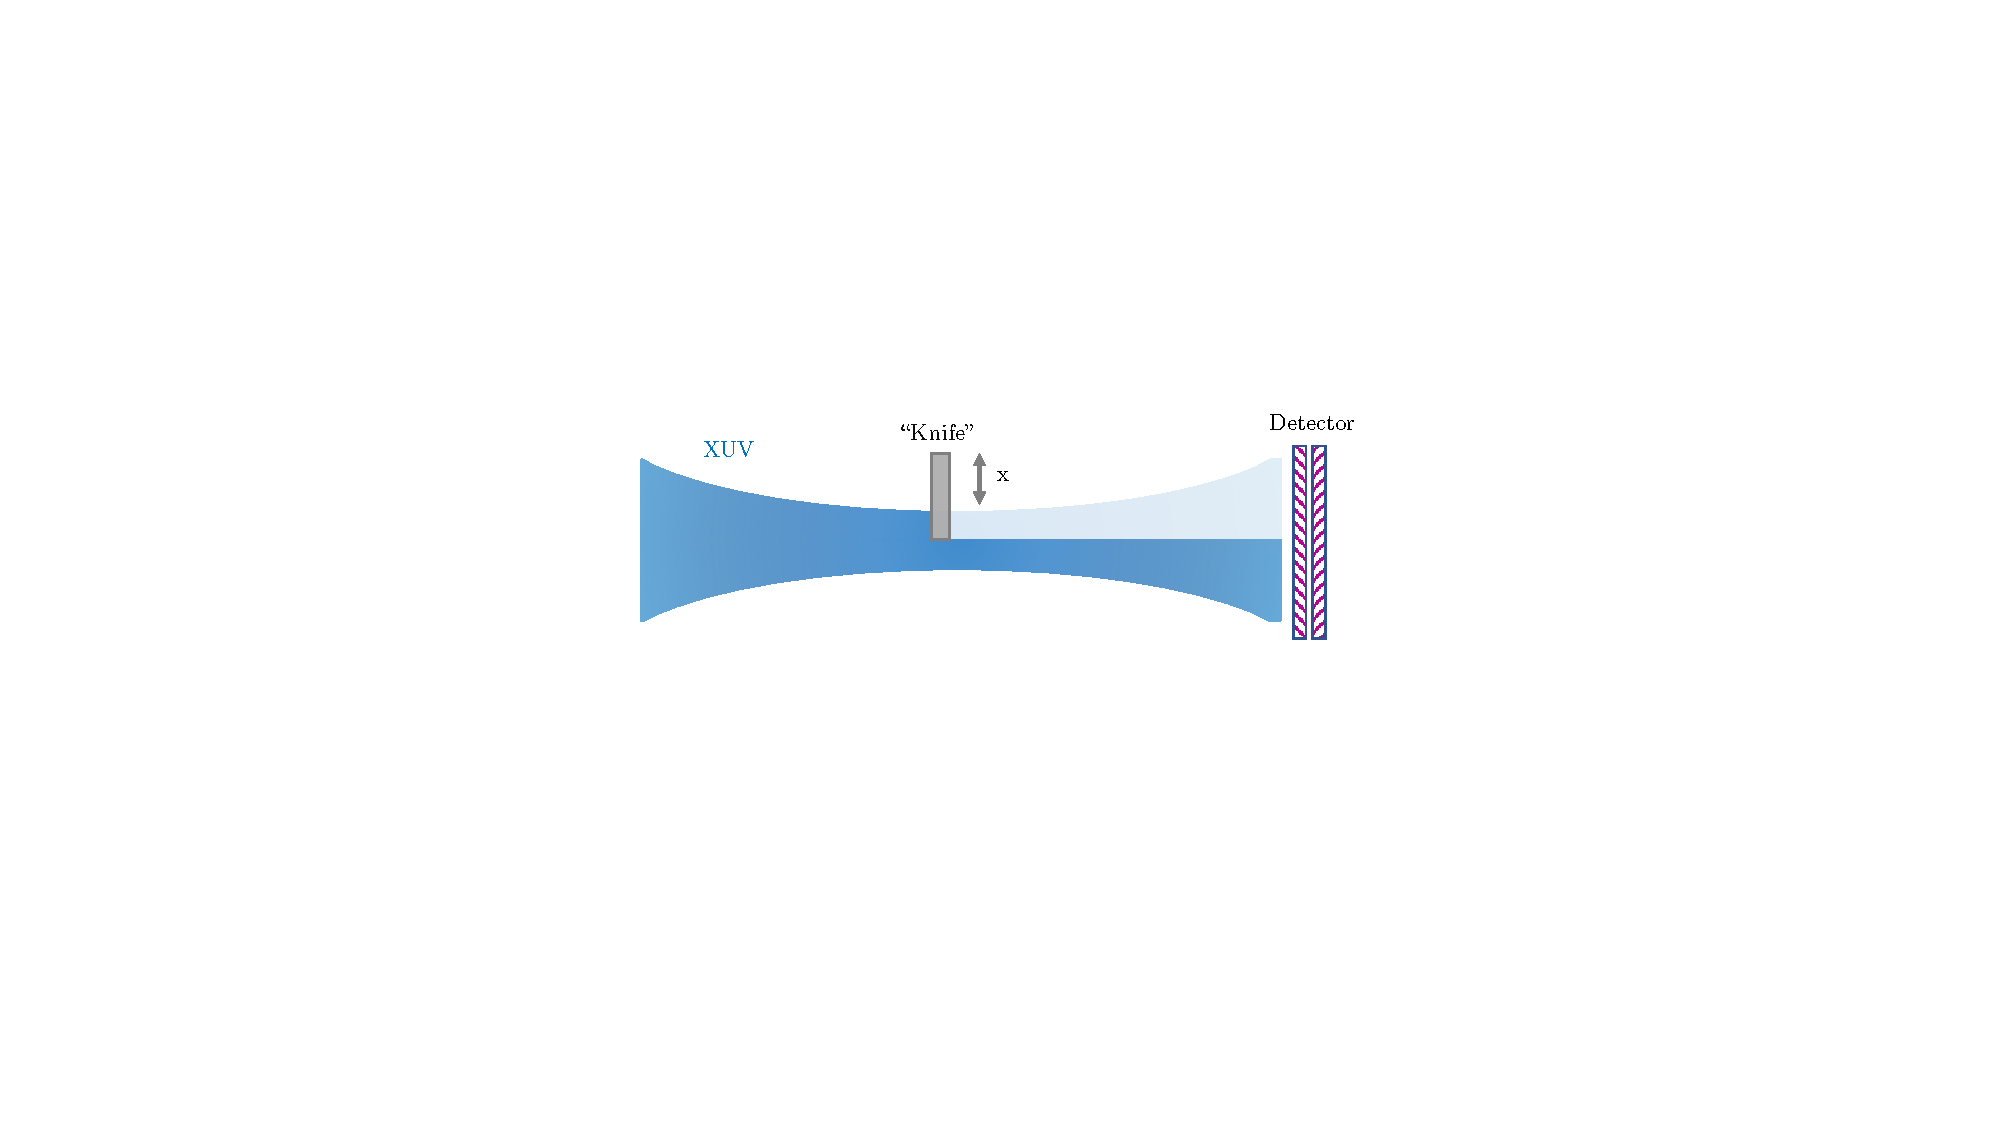
\includegraphics[width=0.7\textwidth]{figures/Beamline/knife_edge_xuv.pdf}
	\caption[Schematic of knife-edge technique to measure beam size]{Schematic of knife-edge technique to measure beam size. By translating a sharp beam block through the focus and measuring the total transmitted power the beam profile can be reconstructed.}
	\label{fig:knife_edge_beam_size_measurement}
\end{figure}

The principle behind the knife-edge measurement is simple, and it is shown schematically in figure \ref{fig:knife_edge_beam_size_measurement}.  In the measurement, a "knife" is translated through the beam to be measured perpendicular to the k-direction of the beam.  The knife is simply an opaque material that has a sharp edge to minimize scattered light.  As this knife is translated through the focus, the total power is measured further downstream as a function of the knife's position within the beam, and this dependence is given by
\begin{equation}
	\label{eqn:knife_edge_power}
	P(x,z) = \int_{-\infty}^{\infty}\int_{-\infty}^{x}I(x', y',z)\diff y\diff x'
\end{equation} 
where $I(x,y,z)$ is the intensity of the beam.  For a Gaussian beam, this relationship becomes
\begin{equation}
	\label{eqn:knife_edge_power_guassian}
	P(x,z) = \frac{P_0}{2}\mathrm{erfc}\bigg(\frac{x\sqrt{2}}{w(z)}\bigg)
\end{equation}
where $w(z)$ is waist radius as a function of $z$ and is given by
\begin{equation}
	\label{eqn:gaussian_waist_radius}
	w(z)=w_0\sqrt{1+\bigg(\frac{z - z_0}{z_R}\bigg)^2}
\end{equation}
where $z_R=\pi w_0^2 n/\lambda$ is the Rayleigh range and $z_0$ is the position of the focus along the k-direction. 

An example of this measurement being used to measure the beam size of the XUV is shown in figure \ref{fig:xuv_beam_size}.  In this case, the knife being used is the beveled edge of a silicon frame that is 300 $\mu$m thick. The thickness of the frame is such that the transmission is negligible through the frame itself.  The integrated harmonic signal is fit to
\begin{equation}
	P(x) = \frac{a}{2}\mathrm{erfc}\bigg(\frac{\sqrt{2}(x-x_0)}{w}\bigg) + b,
\end{equation}
and the beam size can be extracted from the fit.  In this case the beam size was 9 $\mu$m at this position of the XUV focus.  Comparing this beam size to the predicted beam size of the IR, we can see that the XUV spot size relative to the IR spot size is roughly three times smaller.

\begin{figure}
	\centering
	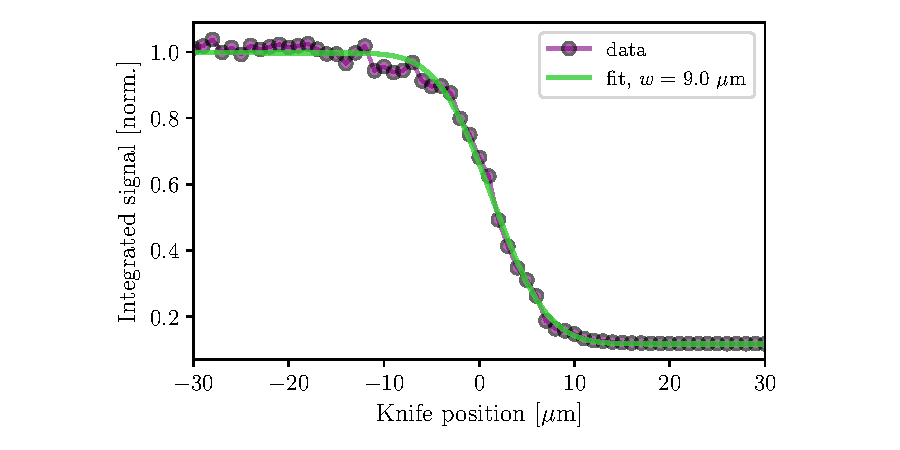
\includegraphics[width=0.9\textwidth]{figures/Beamline/integrated_knife_edge_xuv.pdf}
	\caption[Schematic of knife-edge technique to measure beam size]{Schematic of knife-edge technique to measure beam size. By translating a sharp beam block through the focus and measuring the total transmitted power the beam profile can be reconstructed.}
	\label{fig:xuv_beam_size}
\end{figure}


This measurement can repeated along the k-direction of the XUV beam, and the focus can be mapped out.  An example of this type of measurement is shown in figure \ref{fig:xuv_focus}.  As can be seen, the fit to a Gaussian agrees quite well with the measure dependence of the beam profile.  The extracted Rayleigh range is 1.1 mm with a waist of 6.1 $\mu$m at a motor position of 12.7 mm along the k-direction.  This type of measurement is performed whenever the optical setup is changed in the generation arm of the interferometer, as it insures that the sample is always at the focus of the XUV.
\begin{figure}
	\centering
	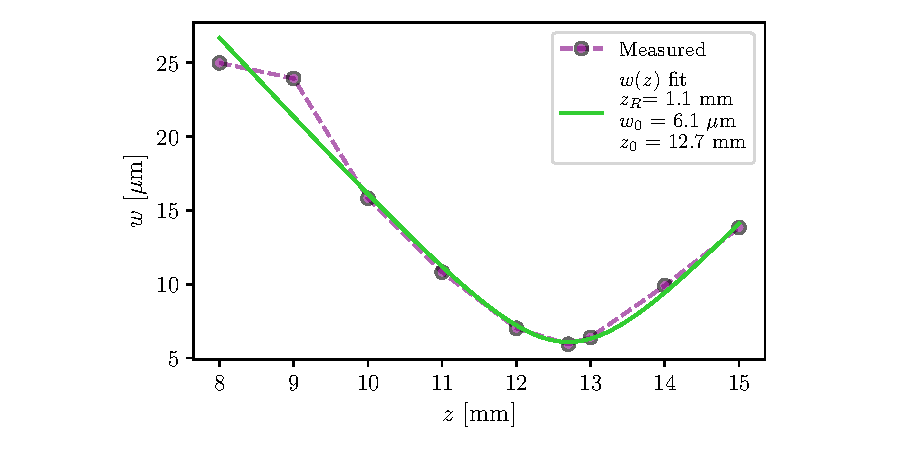
\includegraphics[width=0.9\textwidth]{figures/Beamline/xuv_focus.pdf}
	\caption[Finding focus of XUV using knife-edge measurements]{Focus of the XUV measured using knife-edge method at various points along the k-direction of the XUV beam.}
	\label{fig:xuv_focus}
\end{figure}

\subsection{Spatial and Temporal Overlap}
\label{sec:temporal_overlap}

\begin{figure}
	\centering
	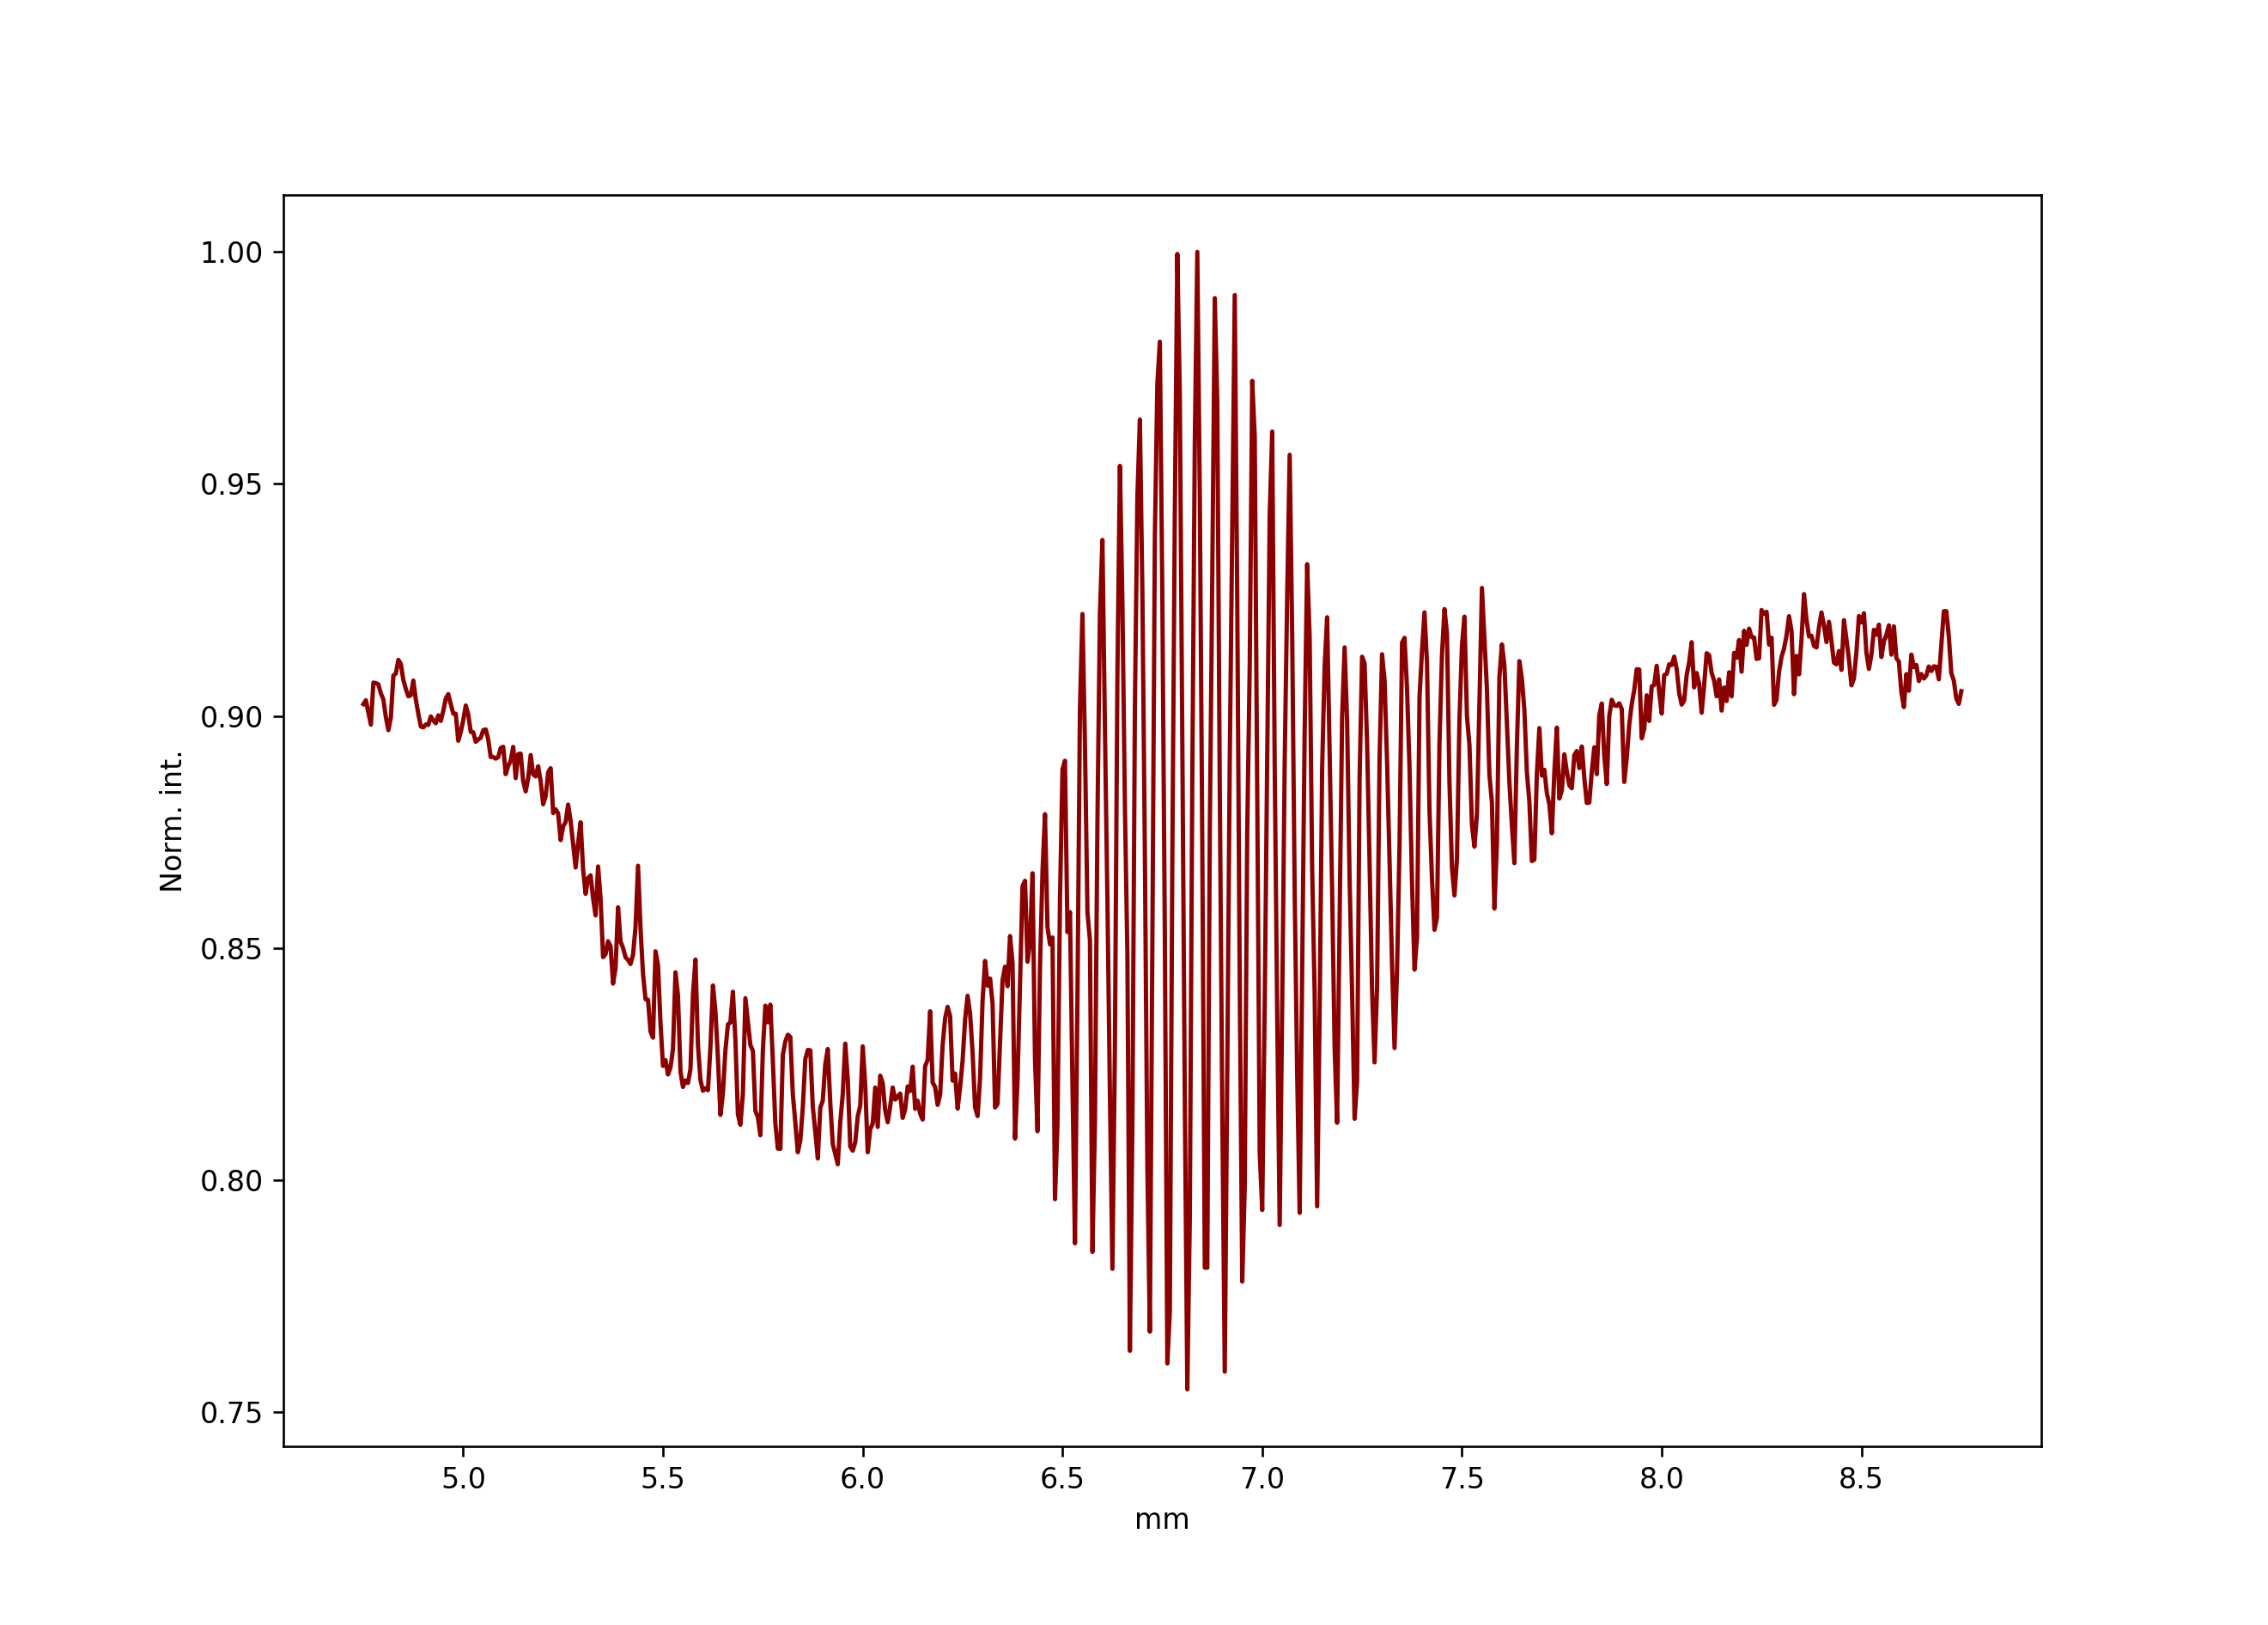
\includegraphics[width=0.9\textwidth]{figures/Beamline/Overlap_camera.png}
	\caption{INCOMPLETE: Autocorrelation to find temporal overlap.}
	\label{fig:fine_scan_temporal_overlap}
\end{figure}

\subsection{Gas Sources for HHG}
\label{sec:gas_source}
\begin{figure}
	\centering
	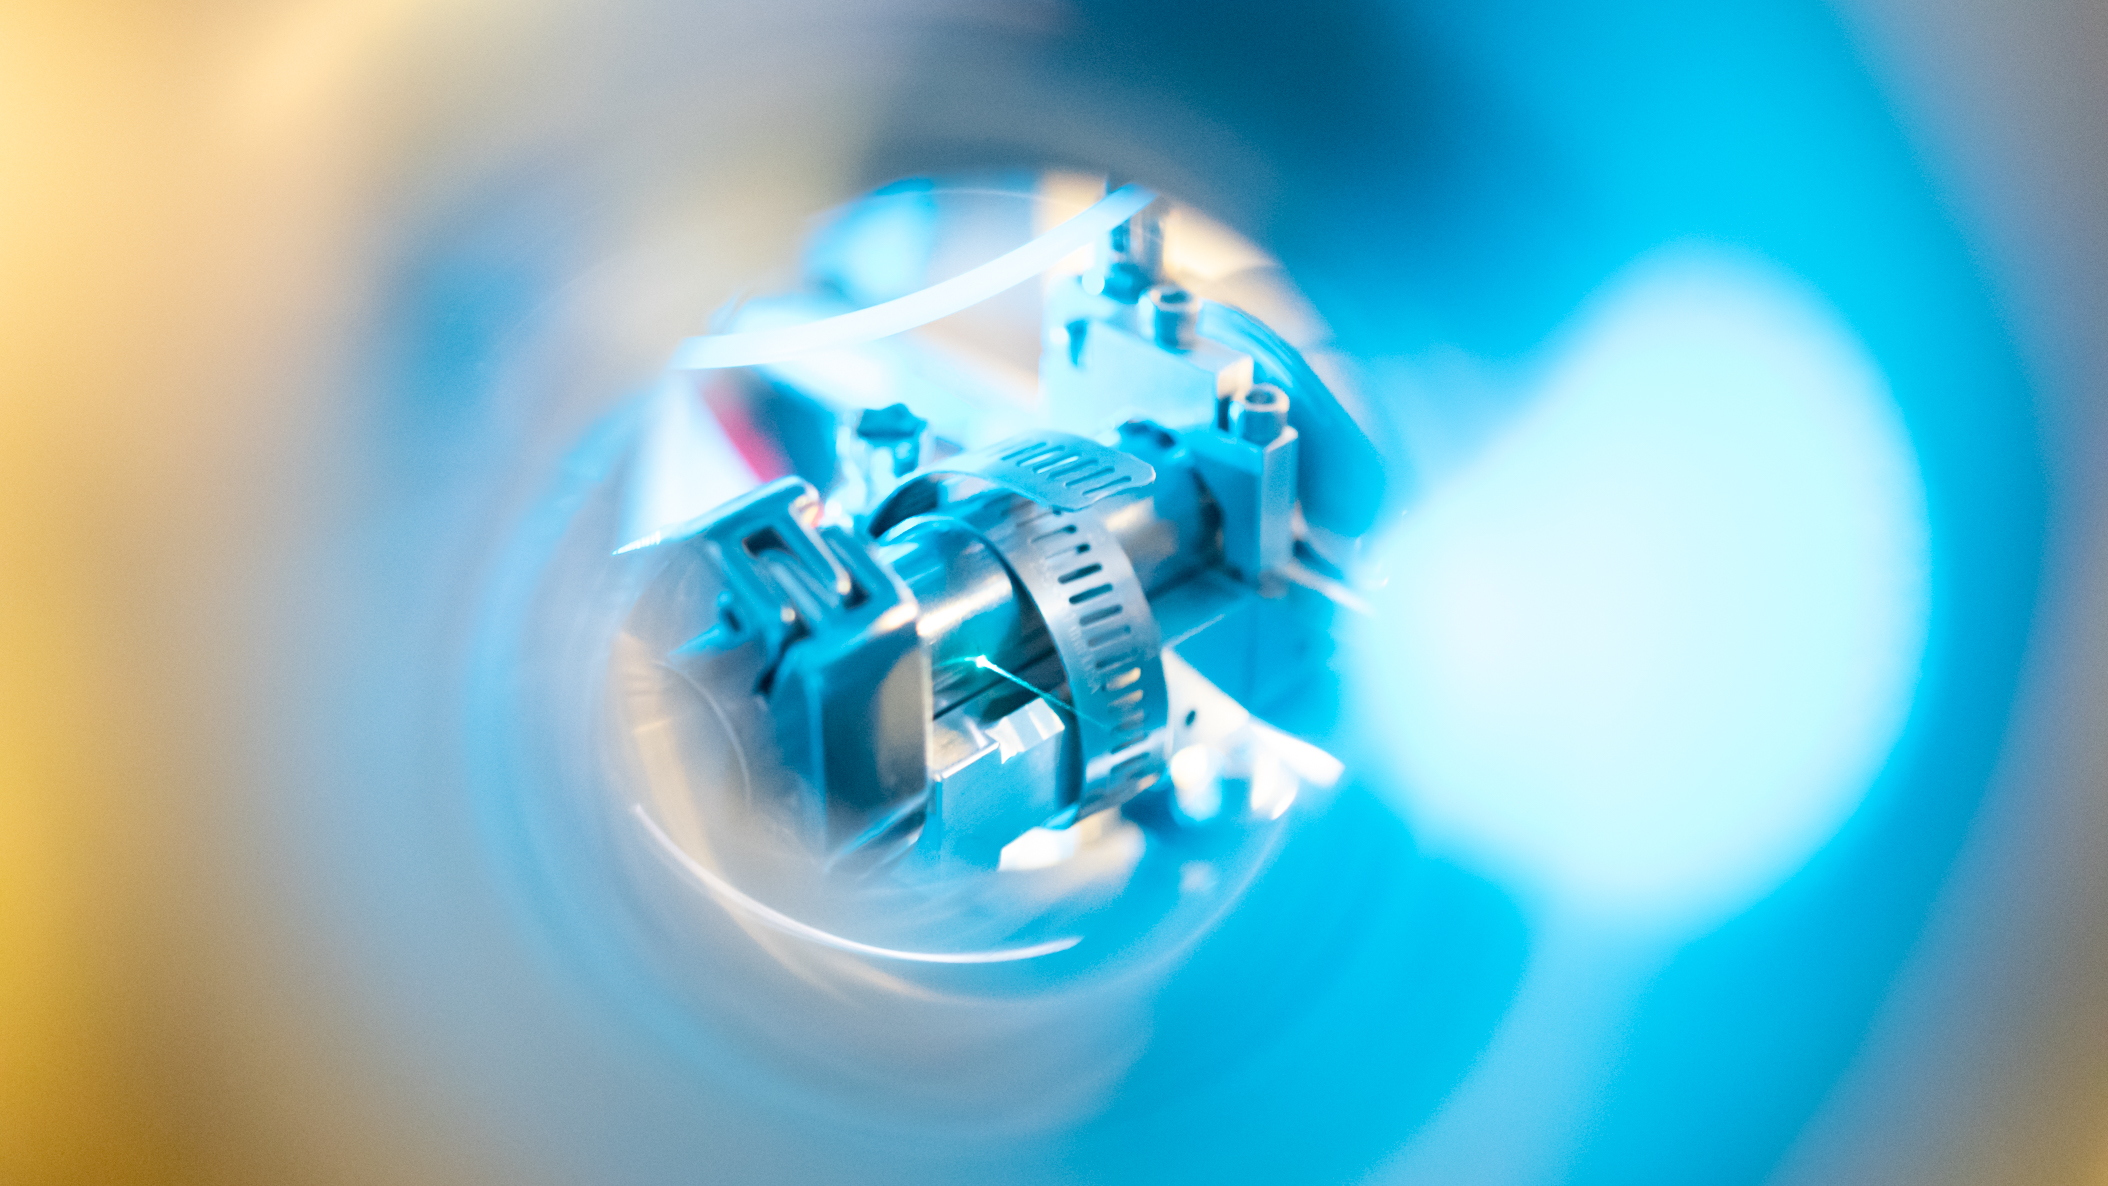
\includegraphics[width=0.9\textwidth]{figures/Beamline/high_pressure_cell_filament.jpg}
	\caption{INCOMPLETE: HPGC filament}
	\label{fig:HPGC_filament}
\end{figure}

\section{Photon Spectrometer}
\label{sec:photon_spec}

\begin{figure}
	\centering
	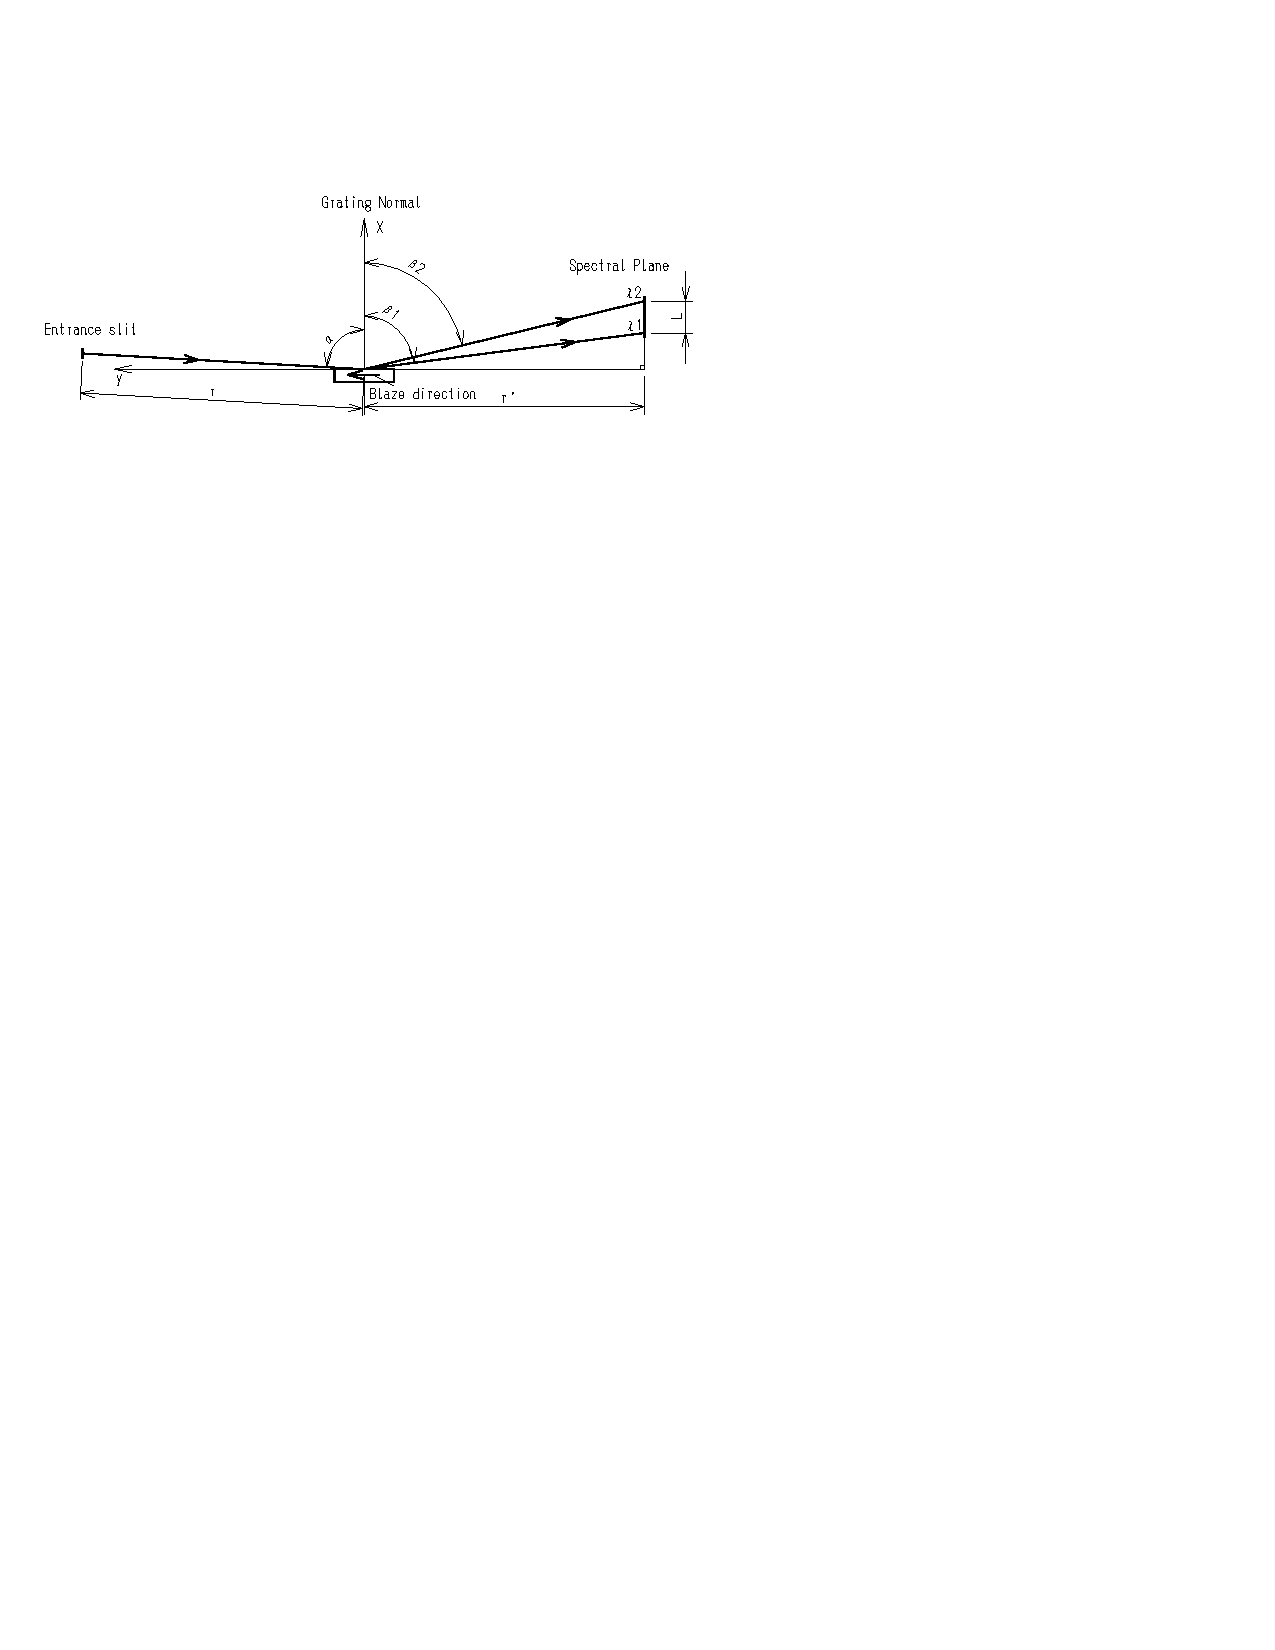
\includegraphics[width=0.9\textwidth]{figures/Beamline/Hitachi.pdf}
	\caption{INCOMPLETE: VLS gratings}
	\label{fig:Hitachi_gratings}
\end{figure}

\subsection{Spectrometer Calibration}
\label{subsec:spec_calibration}

\begin{figure}
	\centering
	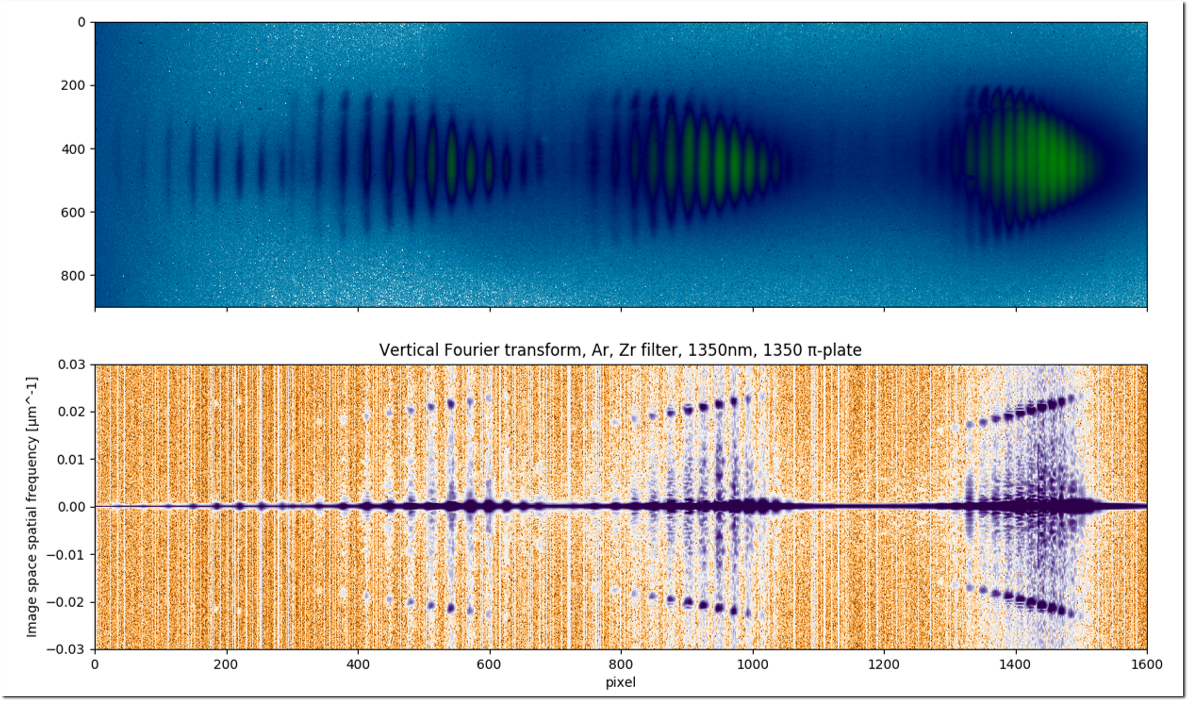
\includegraphics[width=0.9\textwidth]{figures/Beamline/first_to_third_order_diffraction.png}
	\caption{INCOMPLETE: multiple diffraction orders}
	\label{fig:first_to_thirds_order}
\end{figure}

\begin{figure}
	\centering
	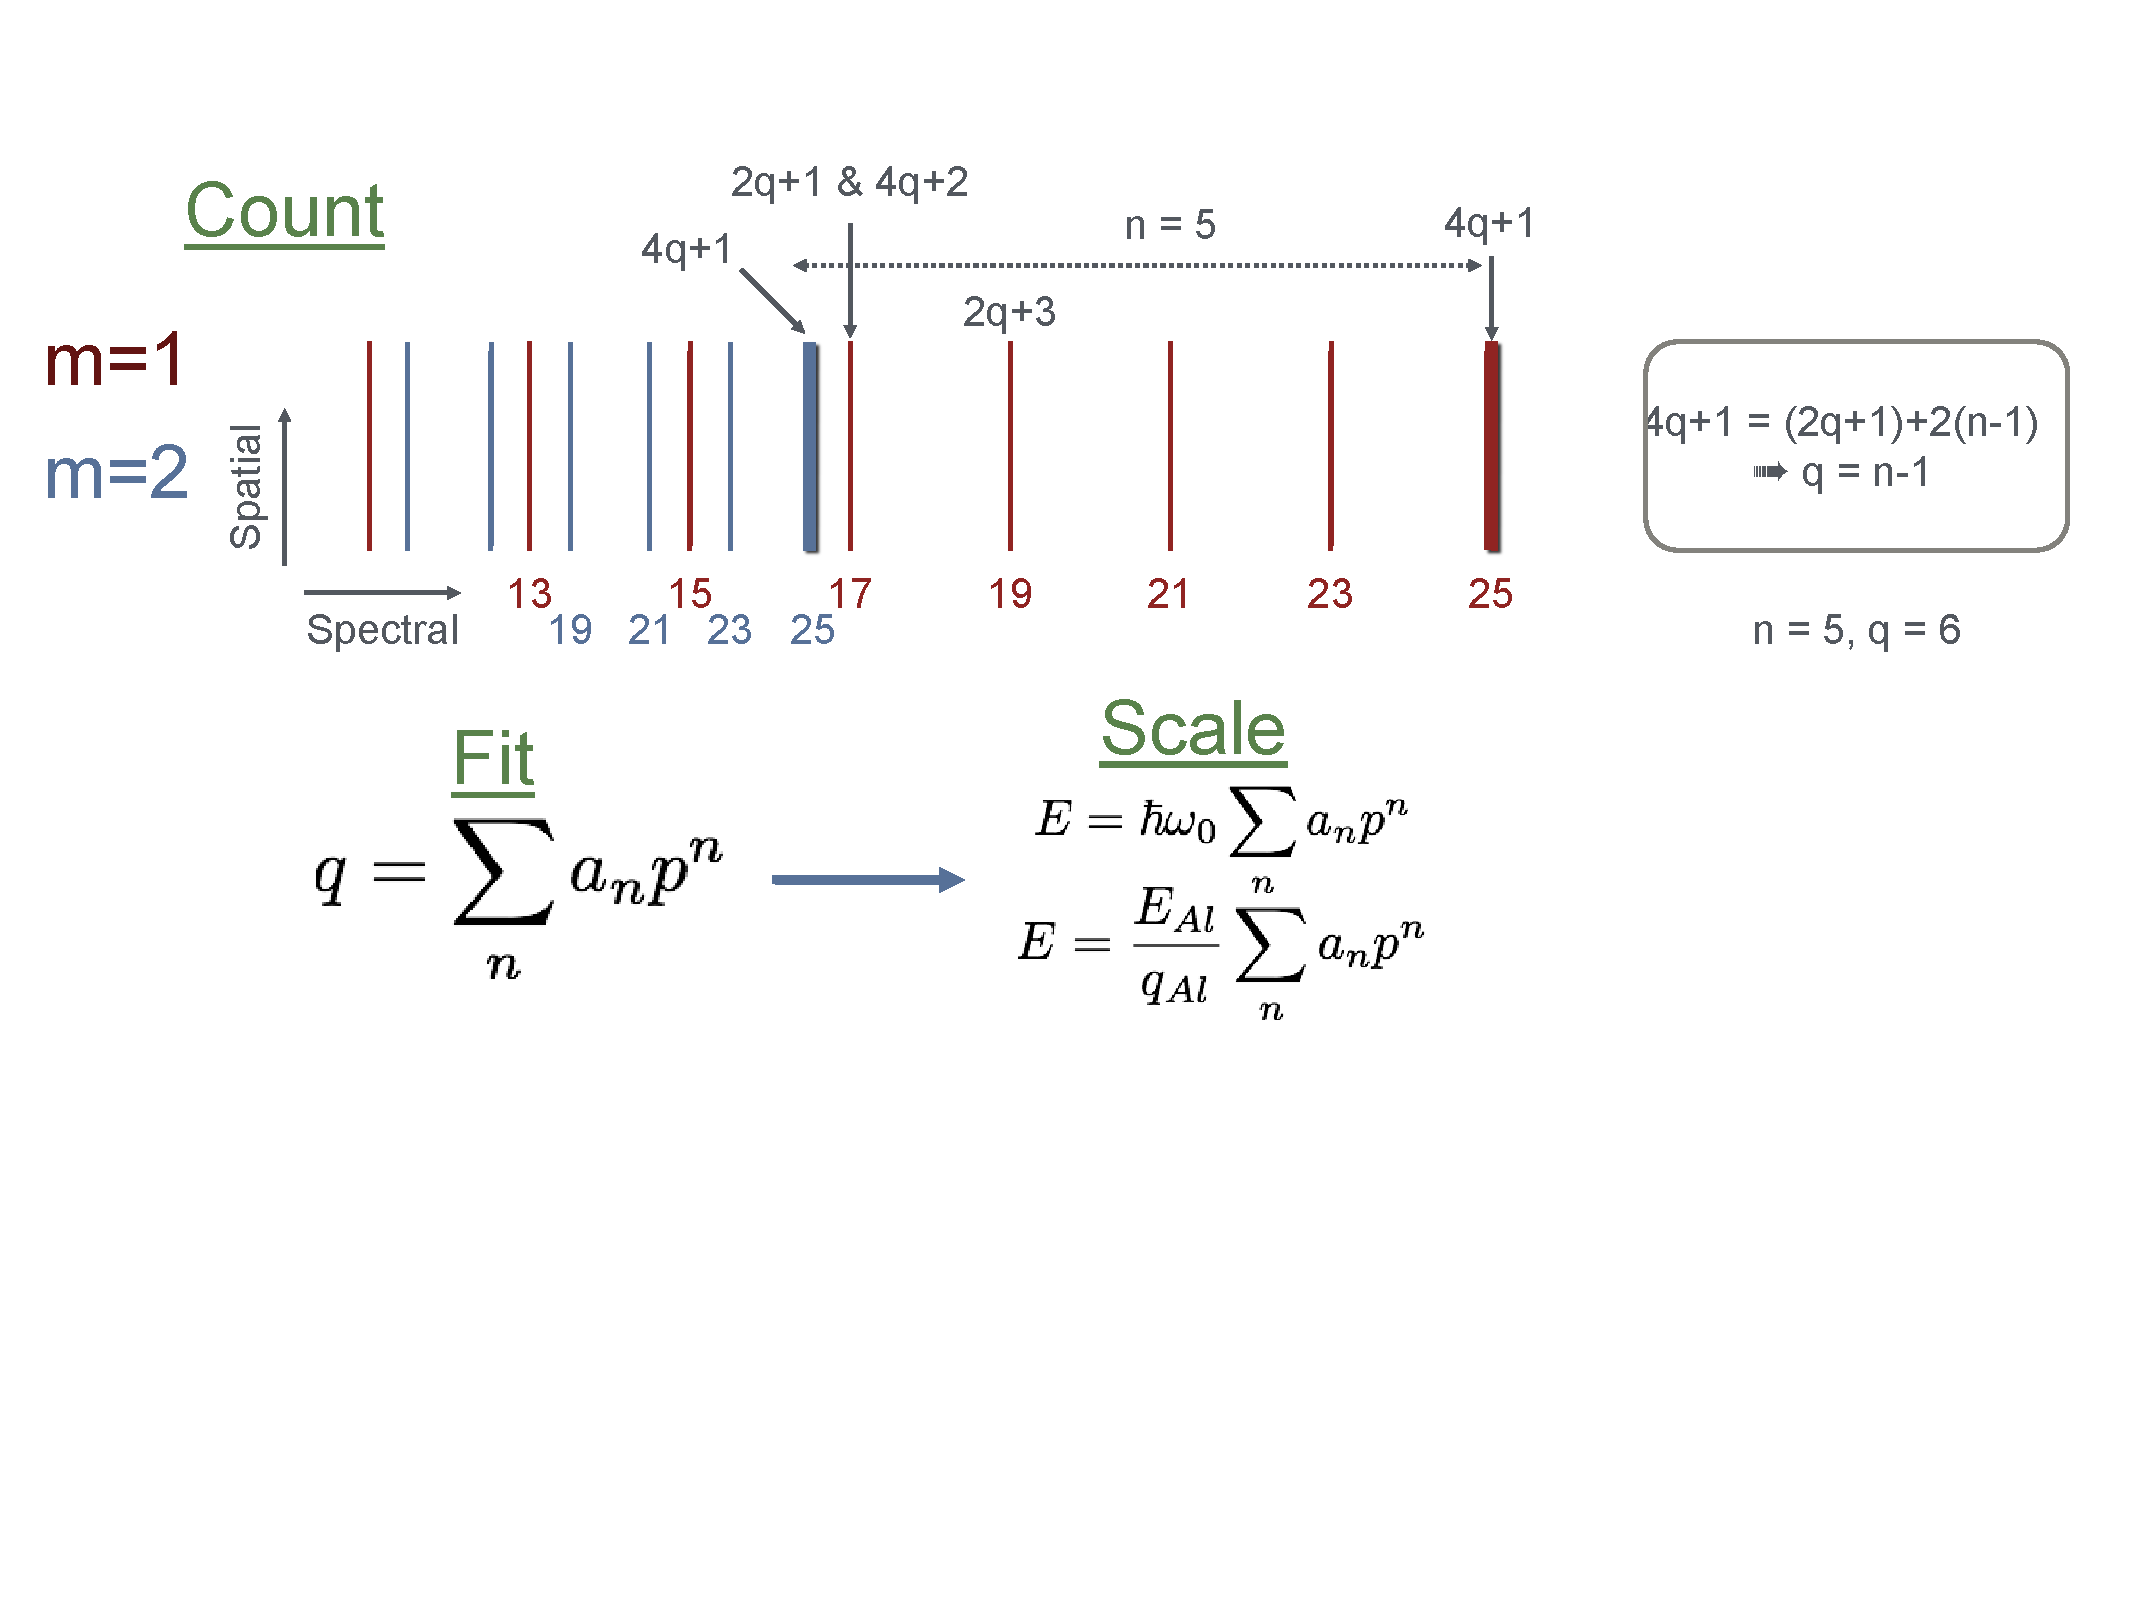
\includegraphics[width=0.9\textwidth]{figures/Beamline/Count_Fit_Scale.pdf}
	\caption{INCOMPLETE: count fit scale scheme}
	\label{fig:count_fit_scale_scheme}
\end{figure}

\begin{figure}
	\centering
	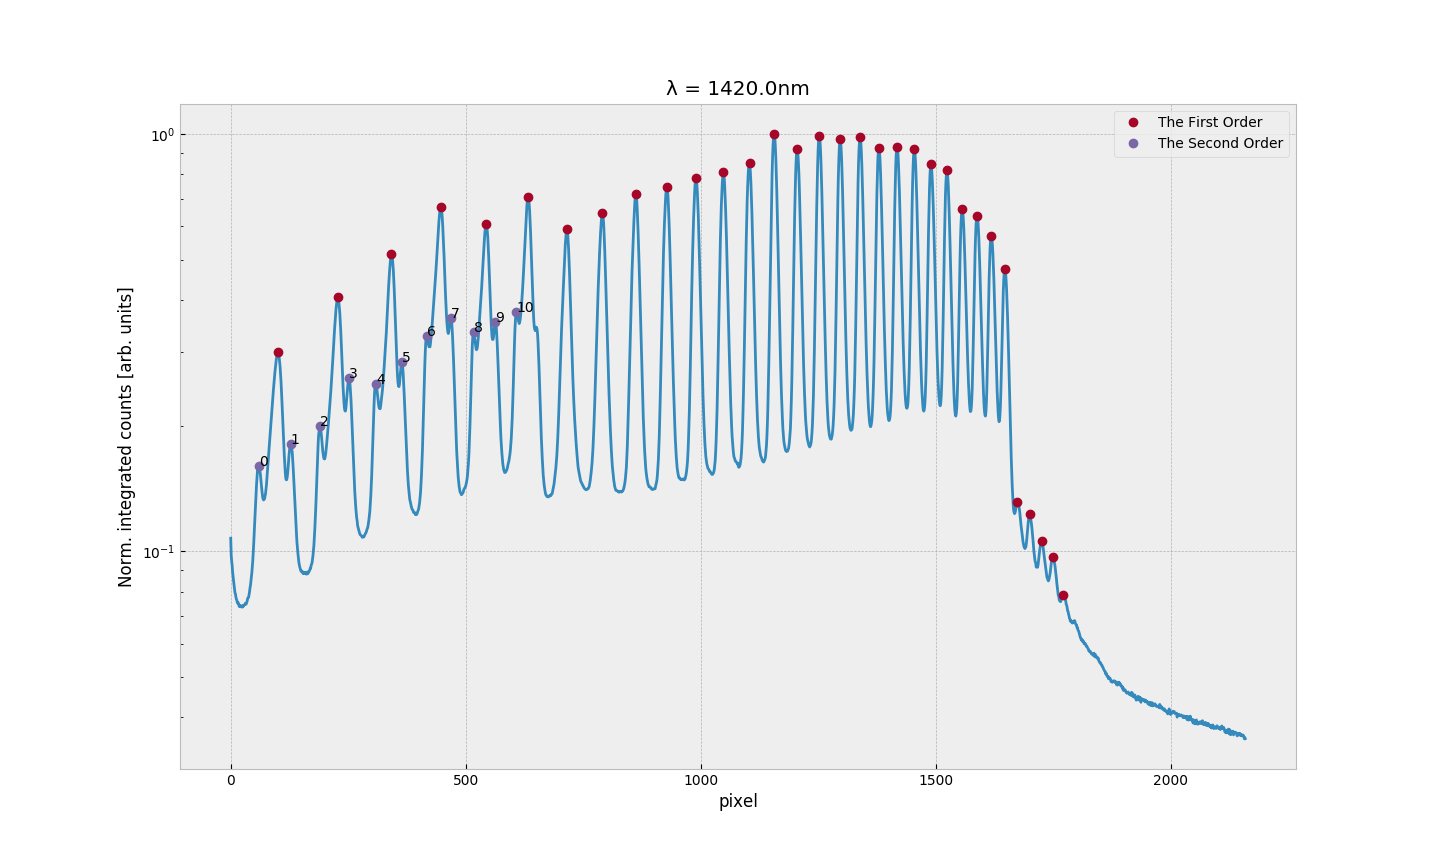
\includegraphics[width=0.9\textwidth]{figures/Beamline/first_second_order_spectrum.png}
	\caption{INCOMPLETE: multiple diffraction orders}
	\label{fig:first_second_order}
\end{figure}

\begin{figure}
	\centering
	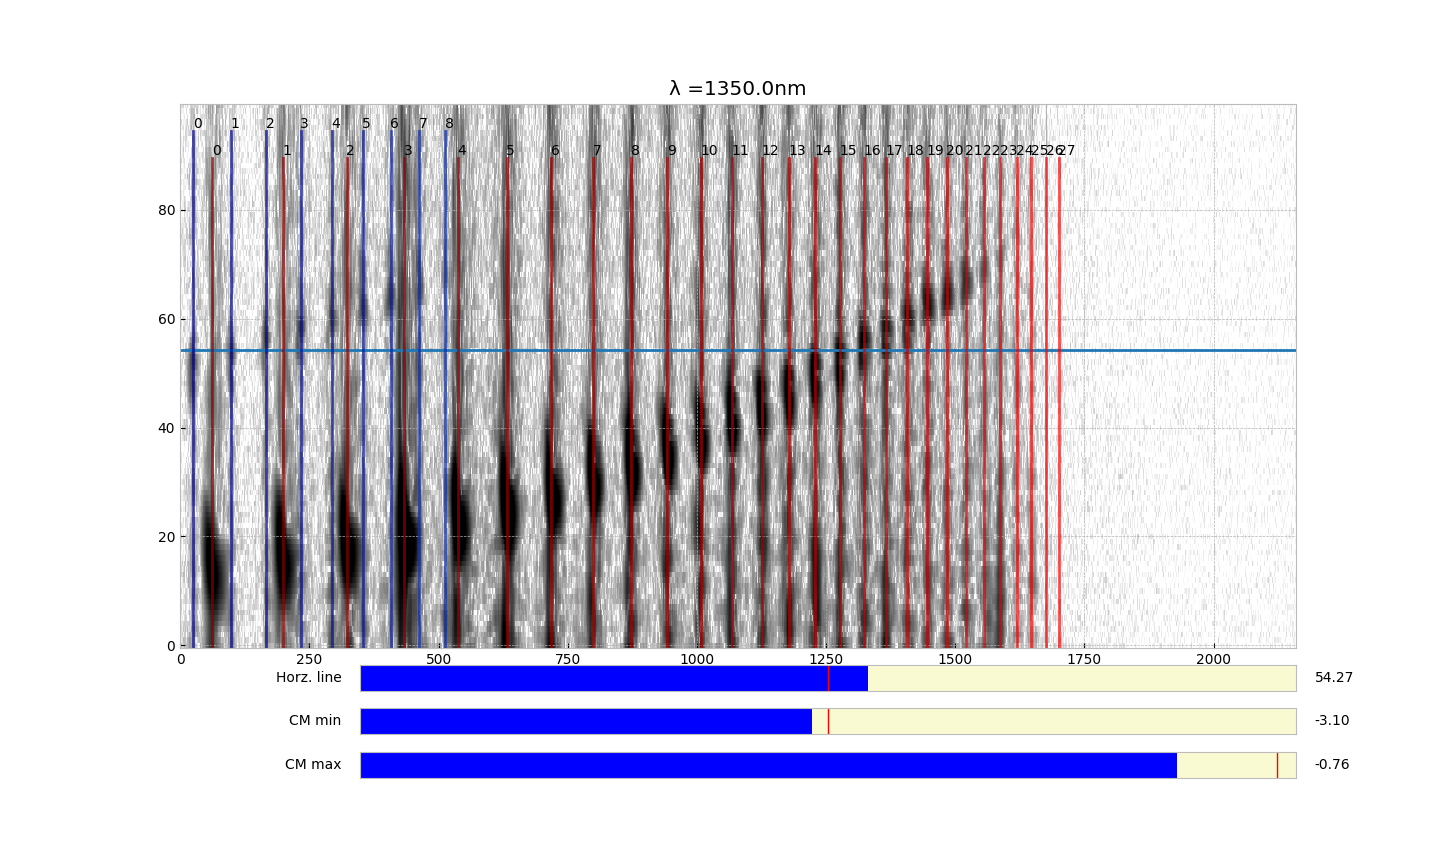
\includegraphics[width=0.9\textwidth]{figures/Beamline/line_matching_first_and_second.png}
	\caption{INCOMPLETE: line matching}
	\label{fig:line_matching}
\end{figure}

\begin{figure}
	\centering
	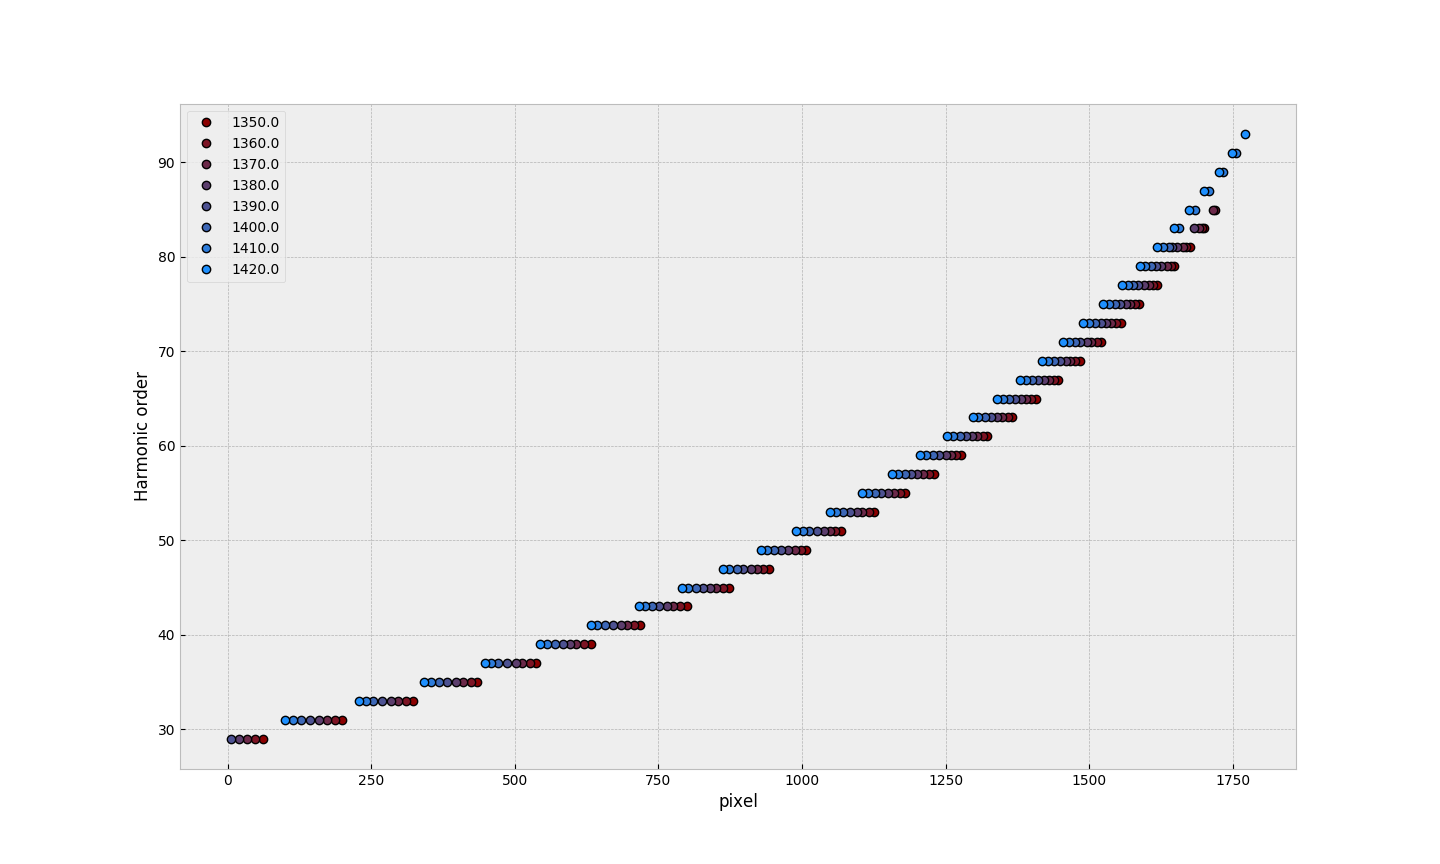
\includegraphics[width=0.9\textwidth]{figures/Beamline/harmonic order vs pixel.png}
	\caption{INCOMPLETE: harmonic order vs pixel}
	\label{fig:harm_order_vs_pixel}
\end{figure}

\begin{figure}
	\centering
	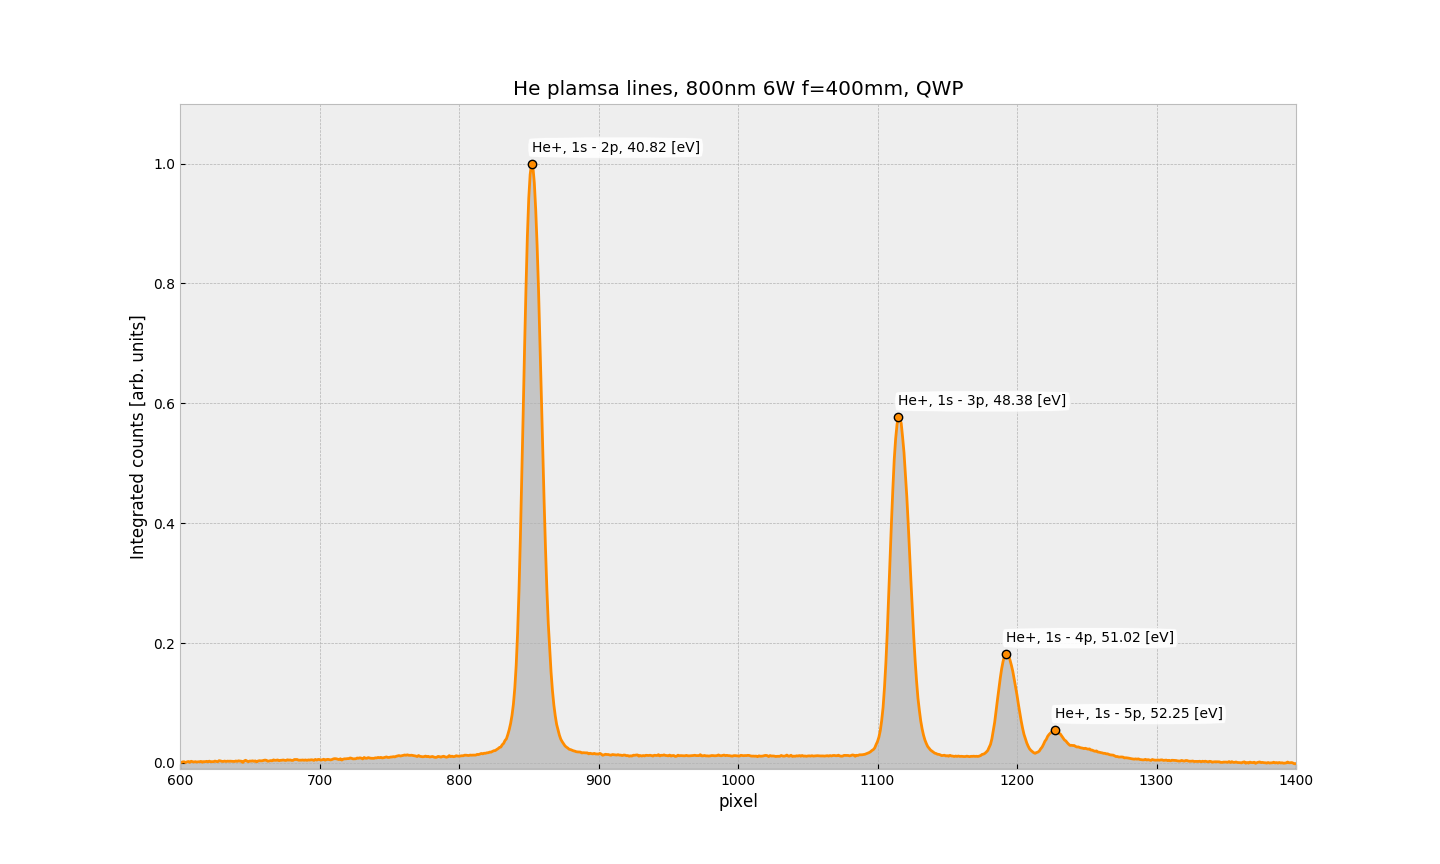
\includegraphics[width=0.9\textwidth]{figures/Beamline/He_plasma_line_spectrum.png}
	\caption{INCOMPLETE: he plasma lines}
	\label{fig:He_plasma_lines}
\end{figure}

\begin{figure}
	\centering
	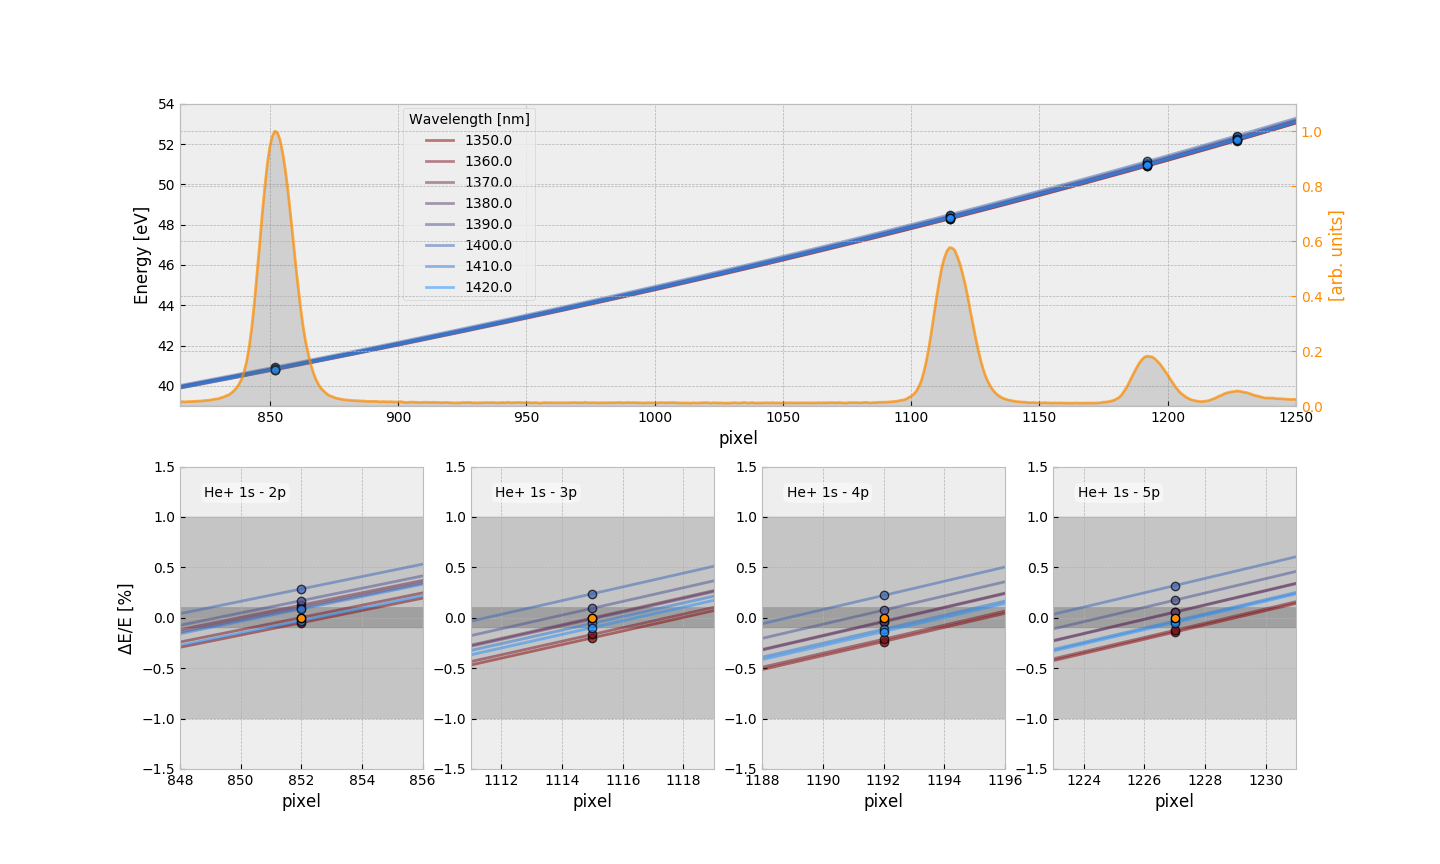
\includegraphics[width=0.9\textwidth]{figures/Beamline/He_plamsa_line_comparison.png}
	\caption{INCOMPLETE: he plasma lines comparison}
	\label{fig:plamsa_line_comparison}
\end{figure}

\begin{figure}
	\centering
	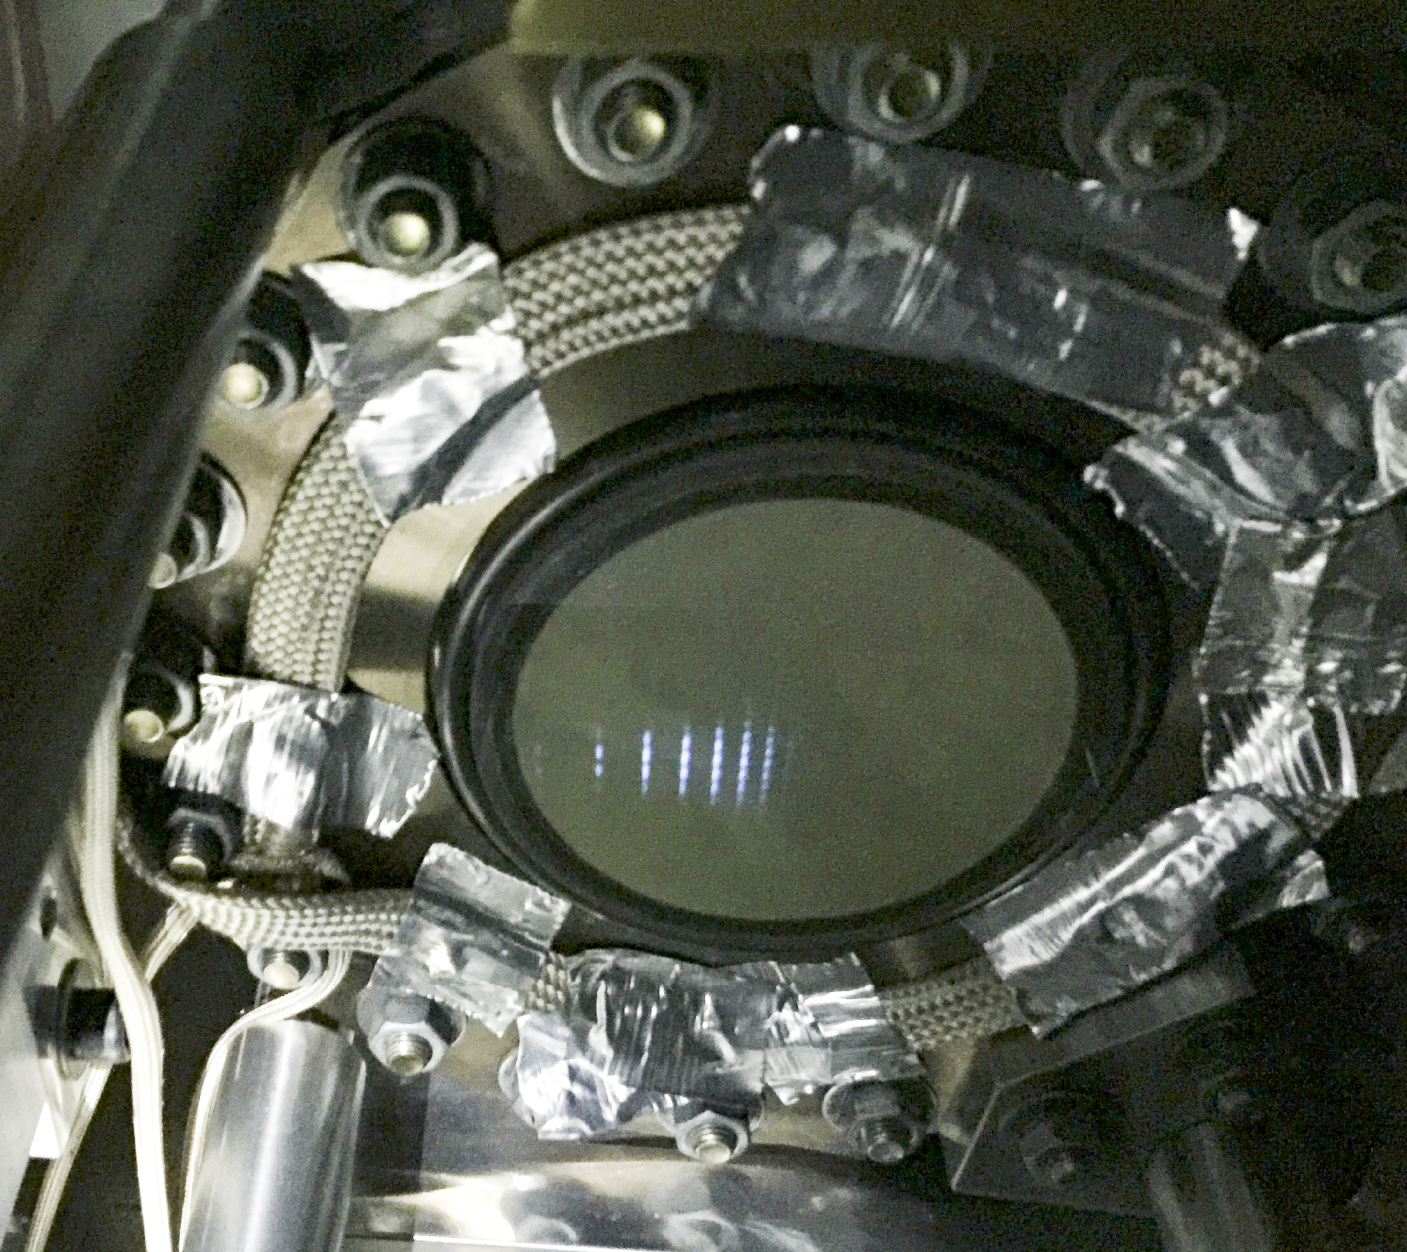
\includegraphics[width=0.6\textwidth]{figures/Two_source/MCP_ts_harmonics.png}
	\caption[Image of phosphor output of high harmonics generated from two sources]{Camera image of the output of the phosphor screen.  Harmonics are visible by eye.}
	\label{MCP_ts_harmonics}
\end{figure}

\begin{figure}
	\centering
	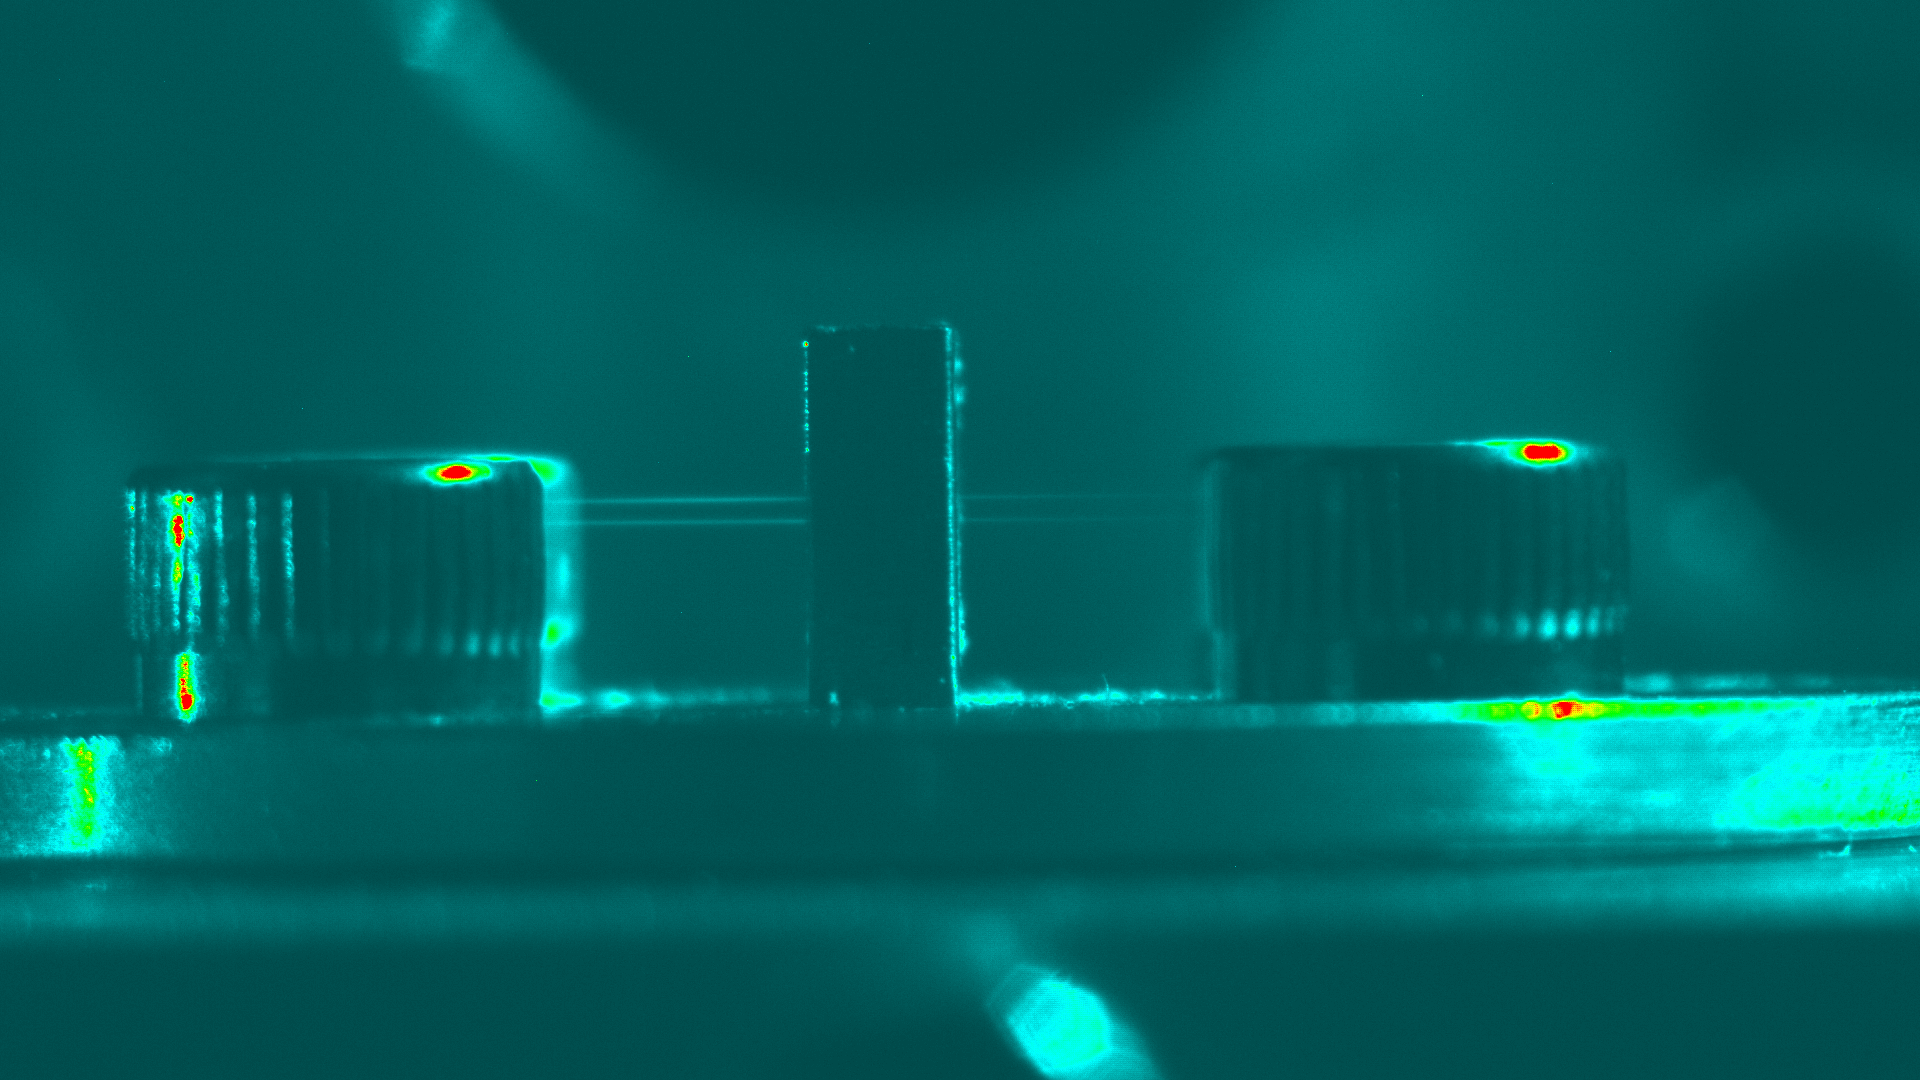
\includegraphics[width=0.9\textwidth]{figures/Two_source/ts_filament_gas_cell.png}
	\caption[Camera image of filaments generated by two sources passing through a gas cell]{Camera image of two sources generating a filament in a gas cell. Image was taken while chamber was vented and at ambient pressure.}
	\label{ts_filament}
\end{figure}

